\subsection{Estatísticas Descritivas}

A \cref{tab:desc} apresenta as estatísticas descritivas das métricas analisadas.

\begin{table}[h]
\centering
\caption{Estatísticas Descritivas}
\label{tab:desc}
\begin{tabular}{lrrrrrrrr}
\toprule
Metrica & Count & Mean & Std & Min & 25\% & Median & 75\% & Max \\
\midrule
files\_changed & 9075.0 & 6.9 & 18.2 & 1.0 & 1.0 & 2.0 & 5.0 & 143.3 \\
lines\_added & 9075.0 & 385.2 & 1512.5 & 0.0 & 2.0 & 20.0 & 124.0 & 12194.7 \\
lines\_deleted & 9075.0 & 94.1 & 414.4 & 0.0 & 1.0 & 3.0 & 19.0 & 3403.7 \\
total\_changes & 9075.0 & 576.2 & 2437.6 & 1.0 & 4.0 & 30.0 & 168.0 & 20171.9 \\
analysis\_time\_hours & 9075.0 & 2105.0 & 6020.9 & 1.2 & 16.6 & 101.6 & 887.8 & 37134.4 \\
description\_chars & 9075.0 & 1320.1 & 1998.3 & 0.0 & 130.0 & 670.0 & 1643.0 & 12038.9 \\
participants & 9075.0 & 3.5 & 1.7 & 2.0 & 2.0 & 3.0 & 4.0 & 11.0 \\
comments\_count & 9075.0 & 0.0 & 0.0 & 0.0 & 0.0 & 0.0 & 0.0 & 0.0 \\
review\_comments\_count & 9075.0 & 0.0 & 0.0 & 0.0 & 0.0 & 0.0 & 0.0 & 0.0 \\
total\_interactions & 9075.0 & 0.0 & 0.0 & 0.0 & 0.0 & 0.0 & 0.0 & 0.0 \\
review\_count & 9075.0 & 2.8 & 3.9 & 1.0 & 1.0 & 1.0 & 3.0 & 26.0 \\
\bottomrule
\end{tabular}

\end{table}

\subsection{Correlações por Questão de Pesquisa}

A \cref{tab:corr} resume os resultados das correlações de \spearman.

\begin{table}[h]
\centering
\caption{Resultados de Correlação}
\label{tab:corr}
\begin{tabular}{lccrrl}
\toprule
RQ & Variavel X & Variavel Y & $\rho$ & p-valor & Efeito \\
\midrule
RQ01 & total\_changes & merged & 0.0034 & 0.7475 & desprezivel \\
RQ02 & analysis\_time\_hours & merged & -0.3910 & 0.0000 & moderada \\
RQ03 & description\_chars & merged & -0.0288 & 0.0061 & desprezivel \\
RQ04 & participants & merged & -0.0756 & 0.0000 & desprezivel \\
RQ05 & total\_changes & review\_count & 0.3114 & 0.0000 & moderada \\
RQ06 & analysis\_time\_hours & review\_count & 0.0917 & 0.0000 & desprezivel \\
RQ07 & description\_chars & review\_count & 0.1861 & 0.0000 & fraca \\
\bottomrule
\end{tabular}

\end{table}

\subsection{Dimensão A: Status do PR}

\subsubsection{RQ01 -- Tamanho vs. Status}
A correlação entre tamanho do PR e status de merge é desprezível
($\rho = 0,0034$, $p = 0,7475$), não significativa.
Medianas idênticas (30 linhas alteradas) para merged e closed.

\begin{figure}[H]
    \centering
    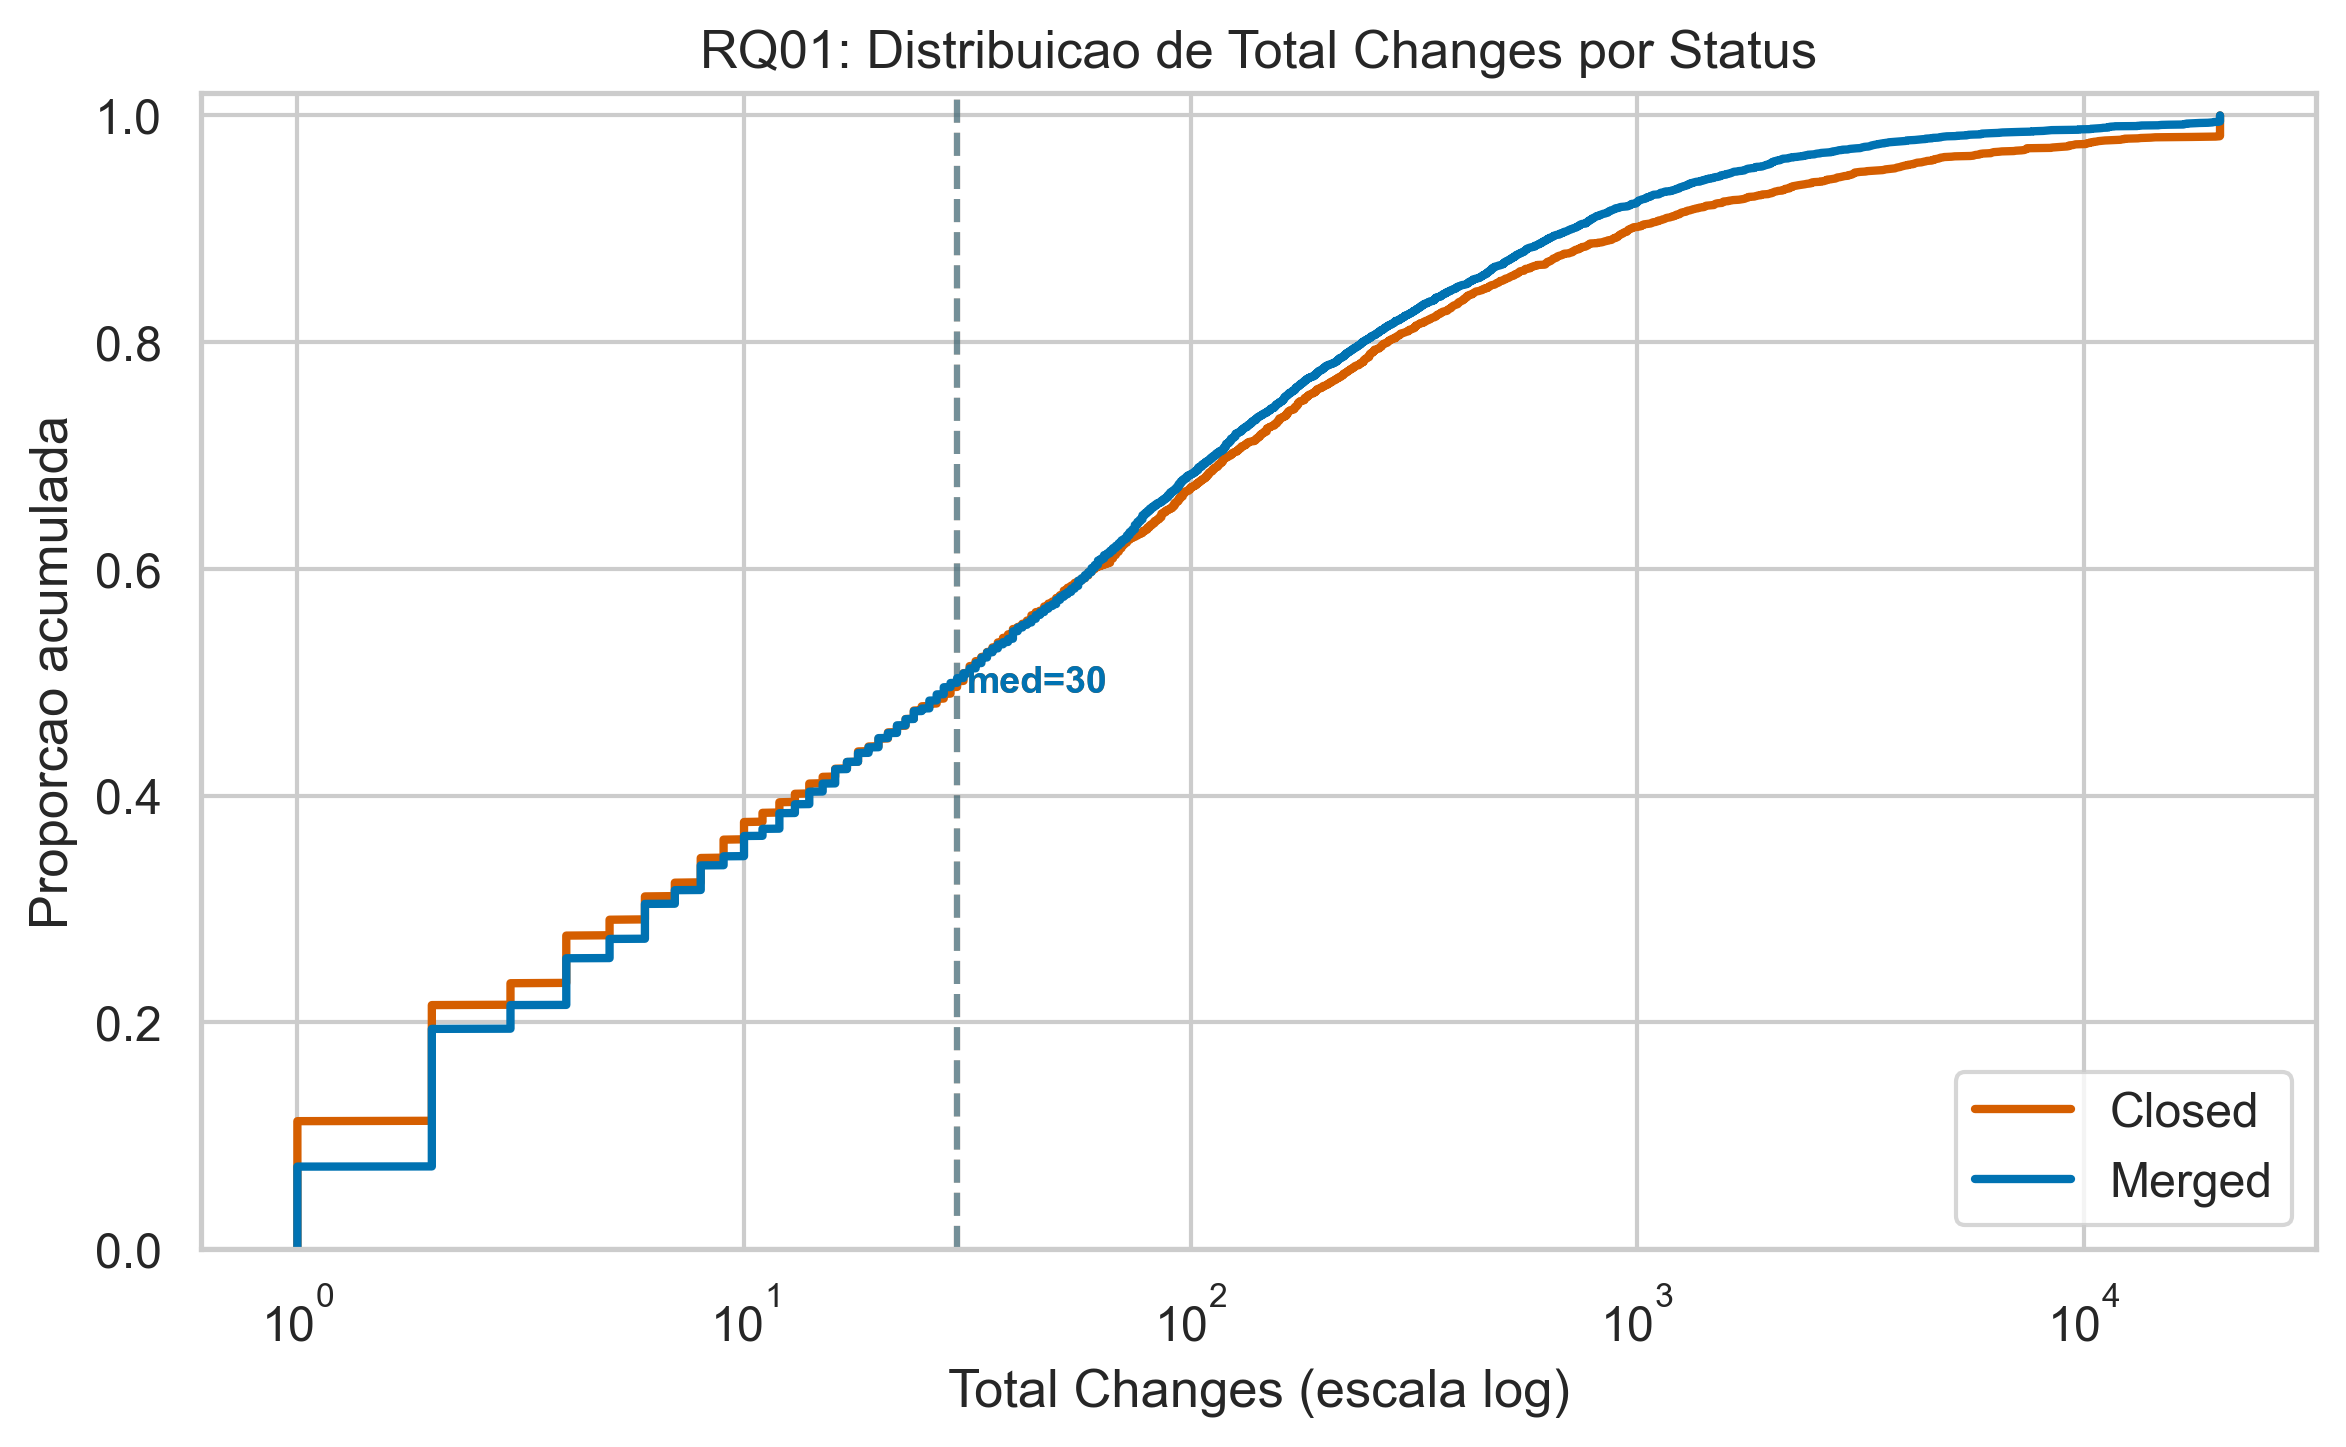
\includegraphics[width=0.85\textwidth]{figures/rq01.png}
    \caption{RQ01: ECDF do tamanho do PR por status de merge.}
    \label{fig:rq01}
\end{figure}

\subsubsection{RQ02 -- Tempo de Análise vs. Status}
Correlação moderada e negativa ($\rho = -0,3910$, $p < 0,0001$).
PRs merged tendem a ter menor tempo de análise: mediana de 47h para merged
vs 748h para closed.

\begin{figure}[H]
    \centering
    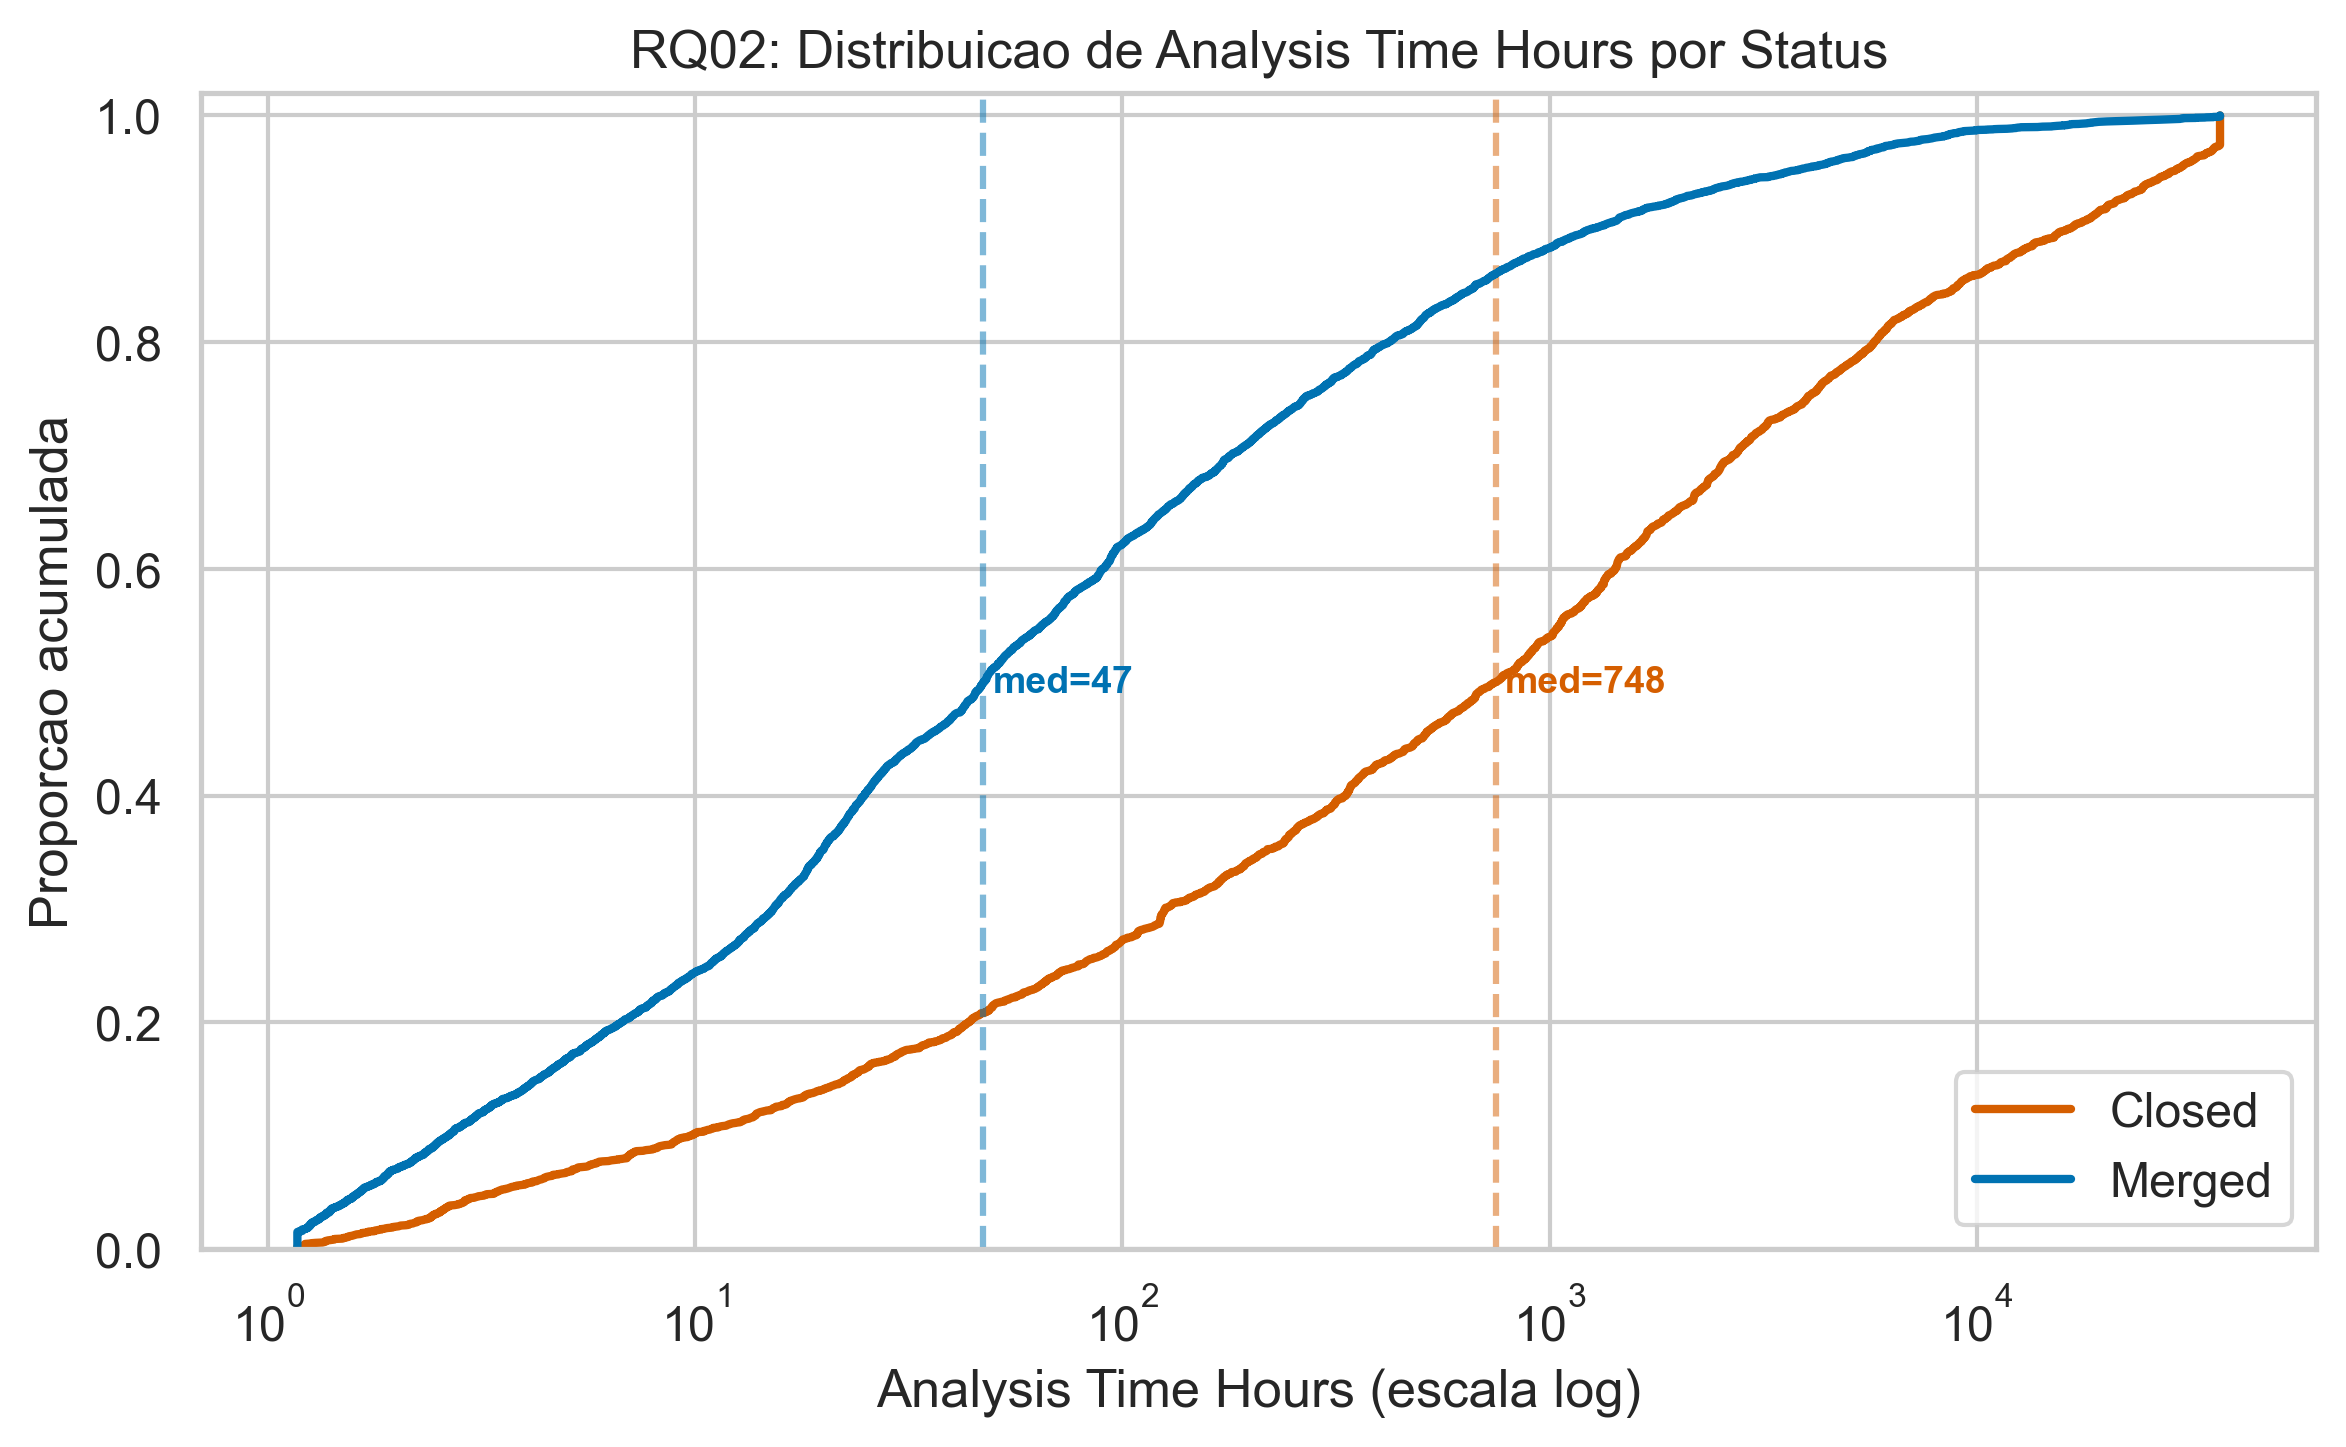
\includegraphics[width=0.85\textwidth]{figures/rq02.png}
    \caption{RQ02: ECDF do tempo de análise por status de merge.}
    \label{fig:rq02}
\end{figure}

\subsubsection{RQ03 -- Descrição vs. Status}
Correlação desprezível ($\rho = -0,0288$, $p = 0,0061$).
Apesar de significativa pelo tamanho da amostra, o efeito é praticamente nulo.

\begin{figure}[H]
    \centering
    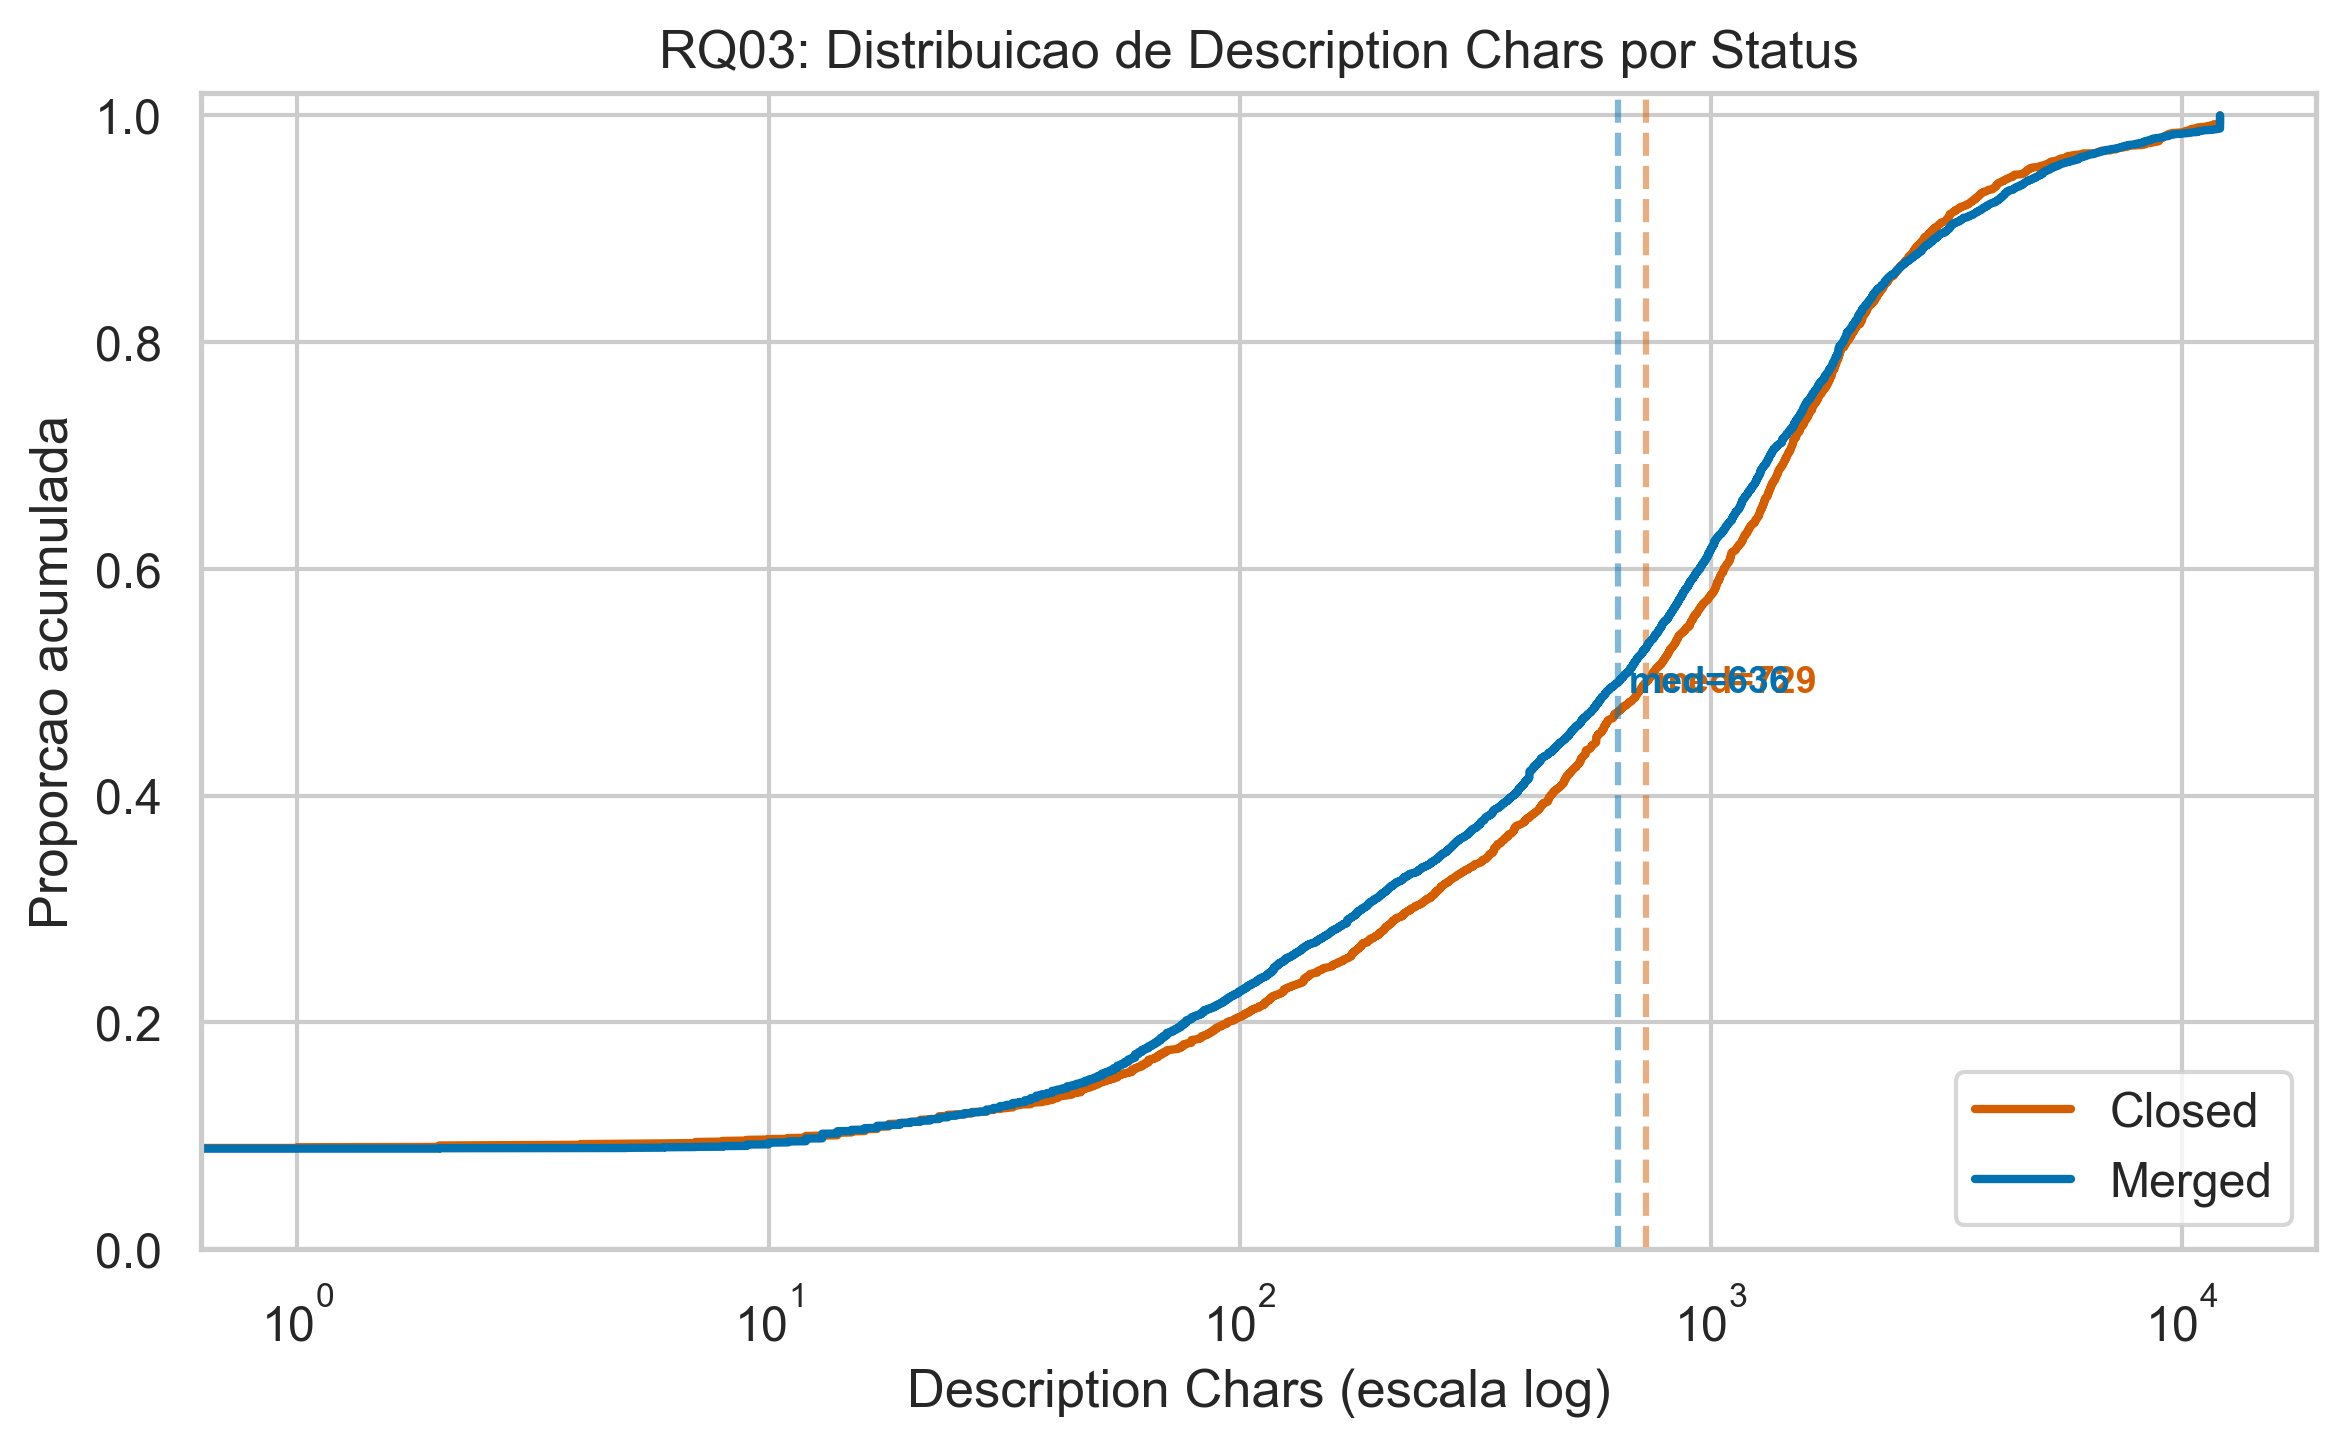
\includegraphics[width=0.85\textwidth]{figures/rq03.png}
    \caption{RQ03: ECDF do tamanho da descrição por status de merge.}
    \label{fig:rq03}
\end{figure}

\subsubsection{RQ04 -- Participantes vs. Status}
Correlação desprezível ($\rho = -0,0756$, $p < 0,0001$).
Mais participantes levemente associados a PRs closed.

\begin{figure}[H]
    \centering
    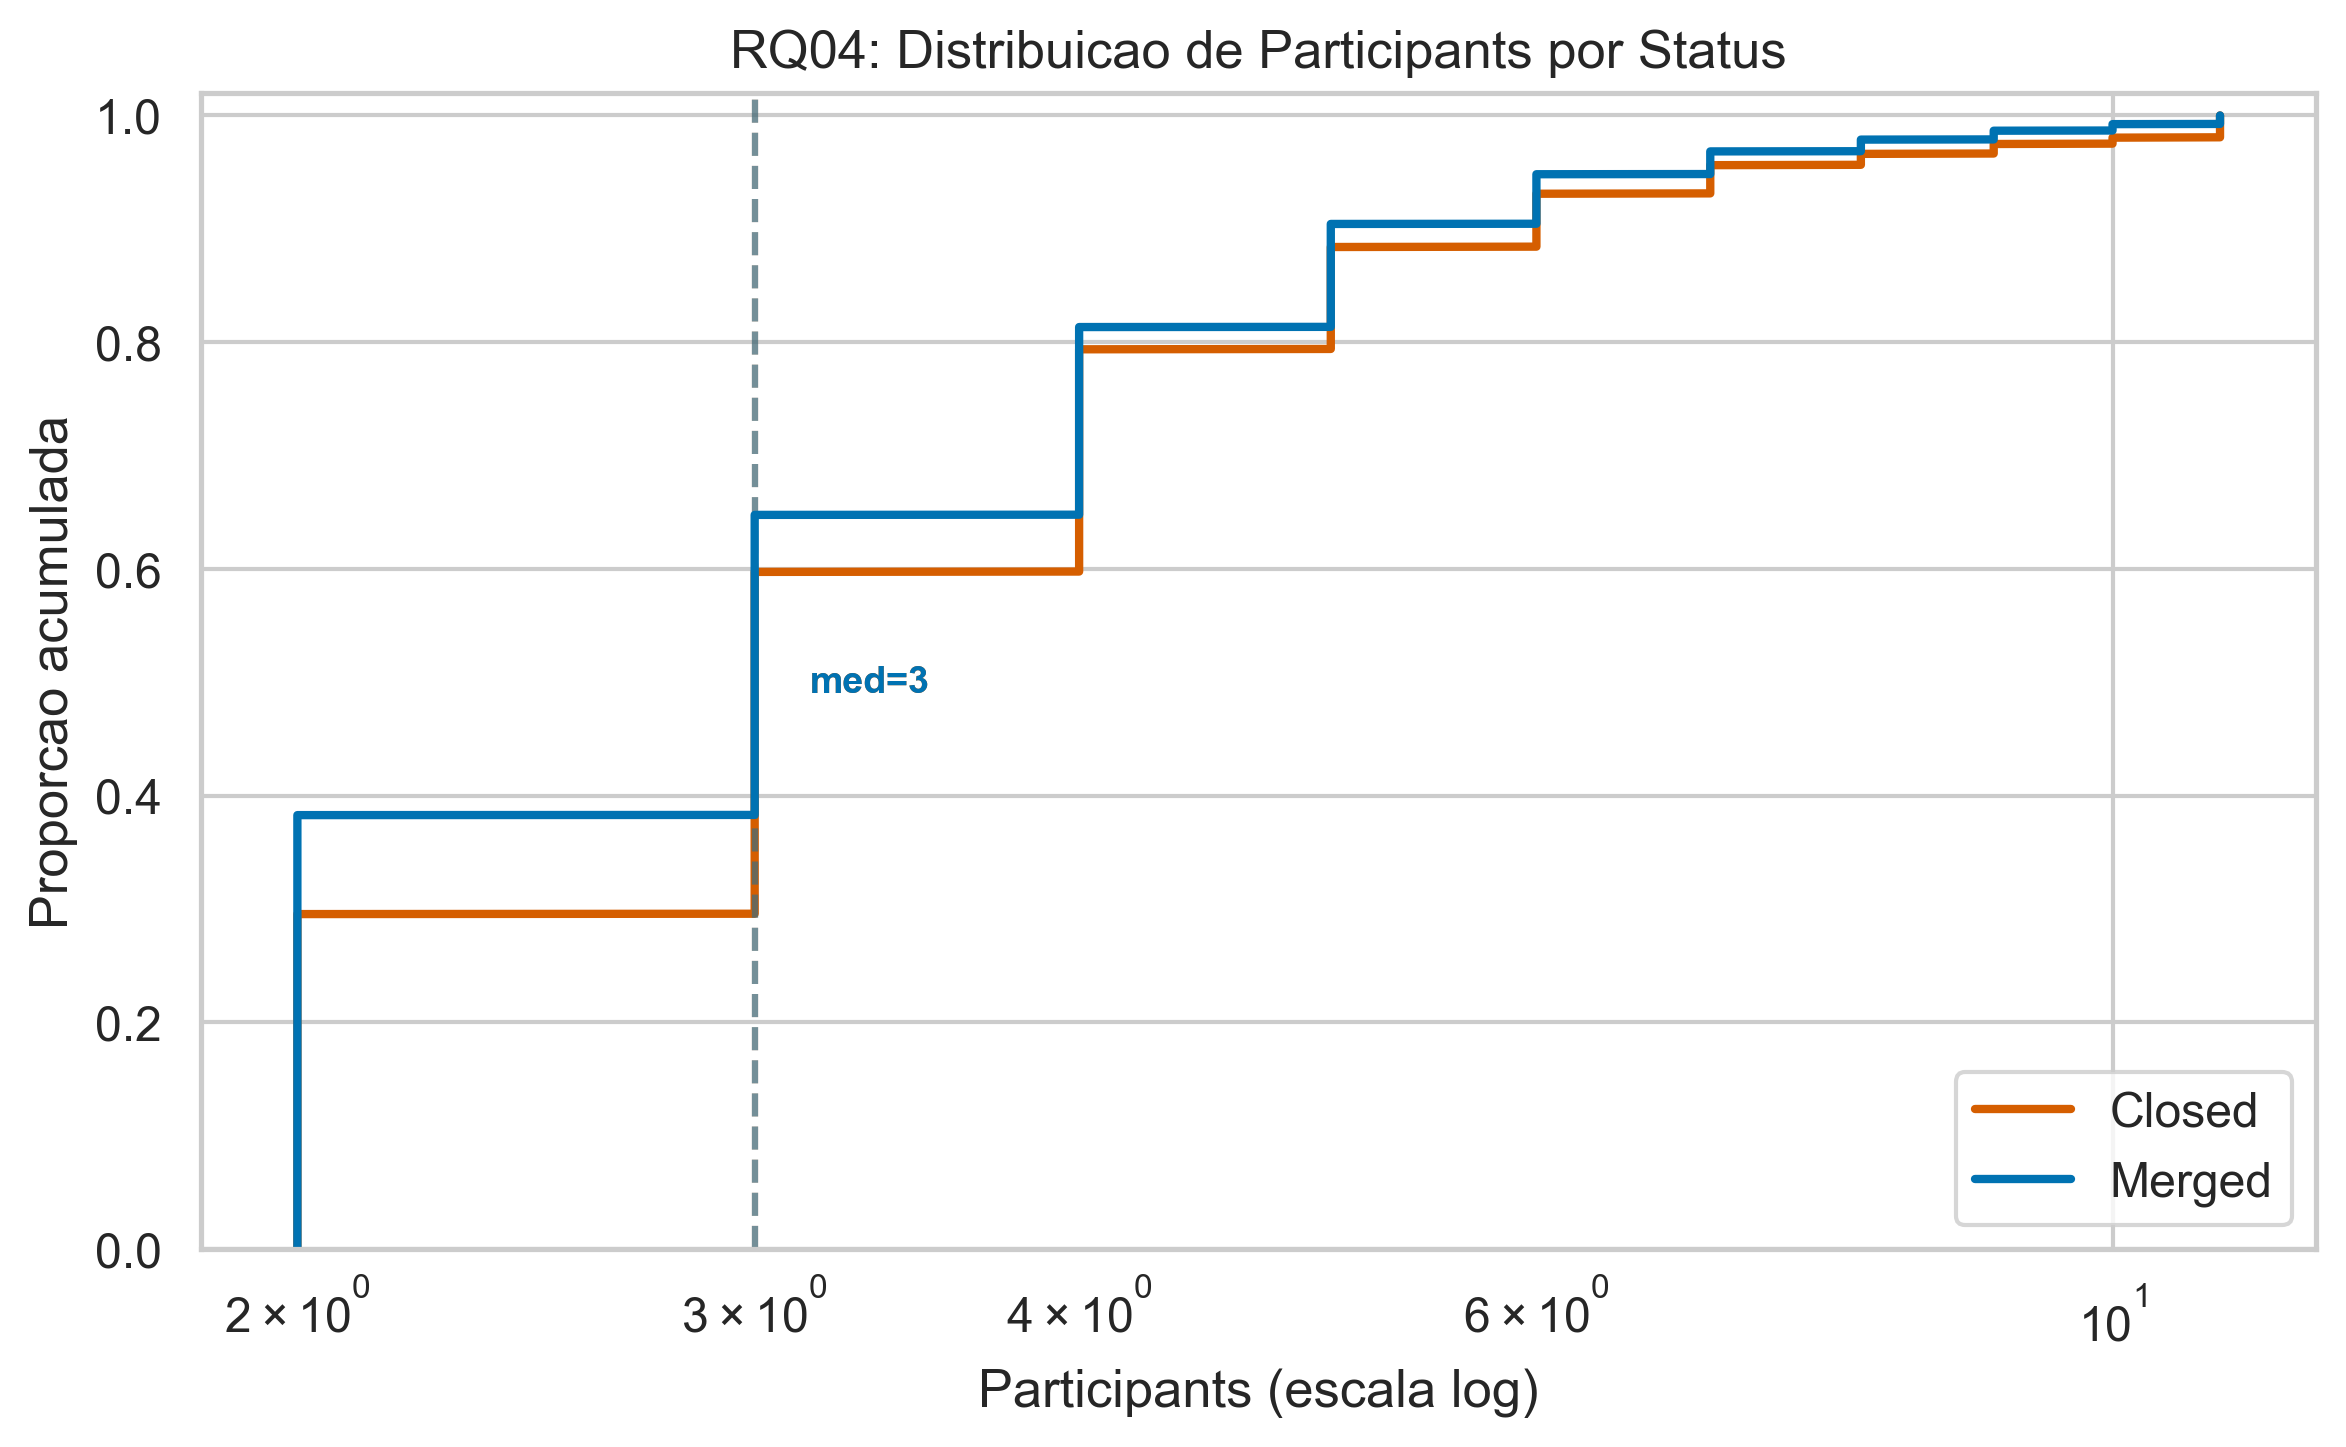
\includegraphics[width=0.85\textwidth]{figures/rq04.png}
    \caption{RQ04: ECDF do número de participantes por status de merge.}
    \label{fig:rq04}
\end{figure}

\subsection{Dimensão B: Número de Revisões}

\subsubsection{RQ05 -- Tamanho vs. Revisões}
Correlação moderada e positiva ($\rho = 0,3114$, $p < 0,0001$).
PRs maiores recebem mais revisões: mediana de 14 linhas (1 revisão)
cresce para 342 (10 revisões).

\begin{figure}[H]
    \centering
    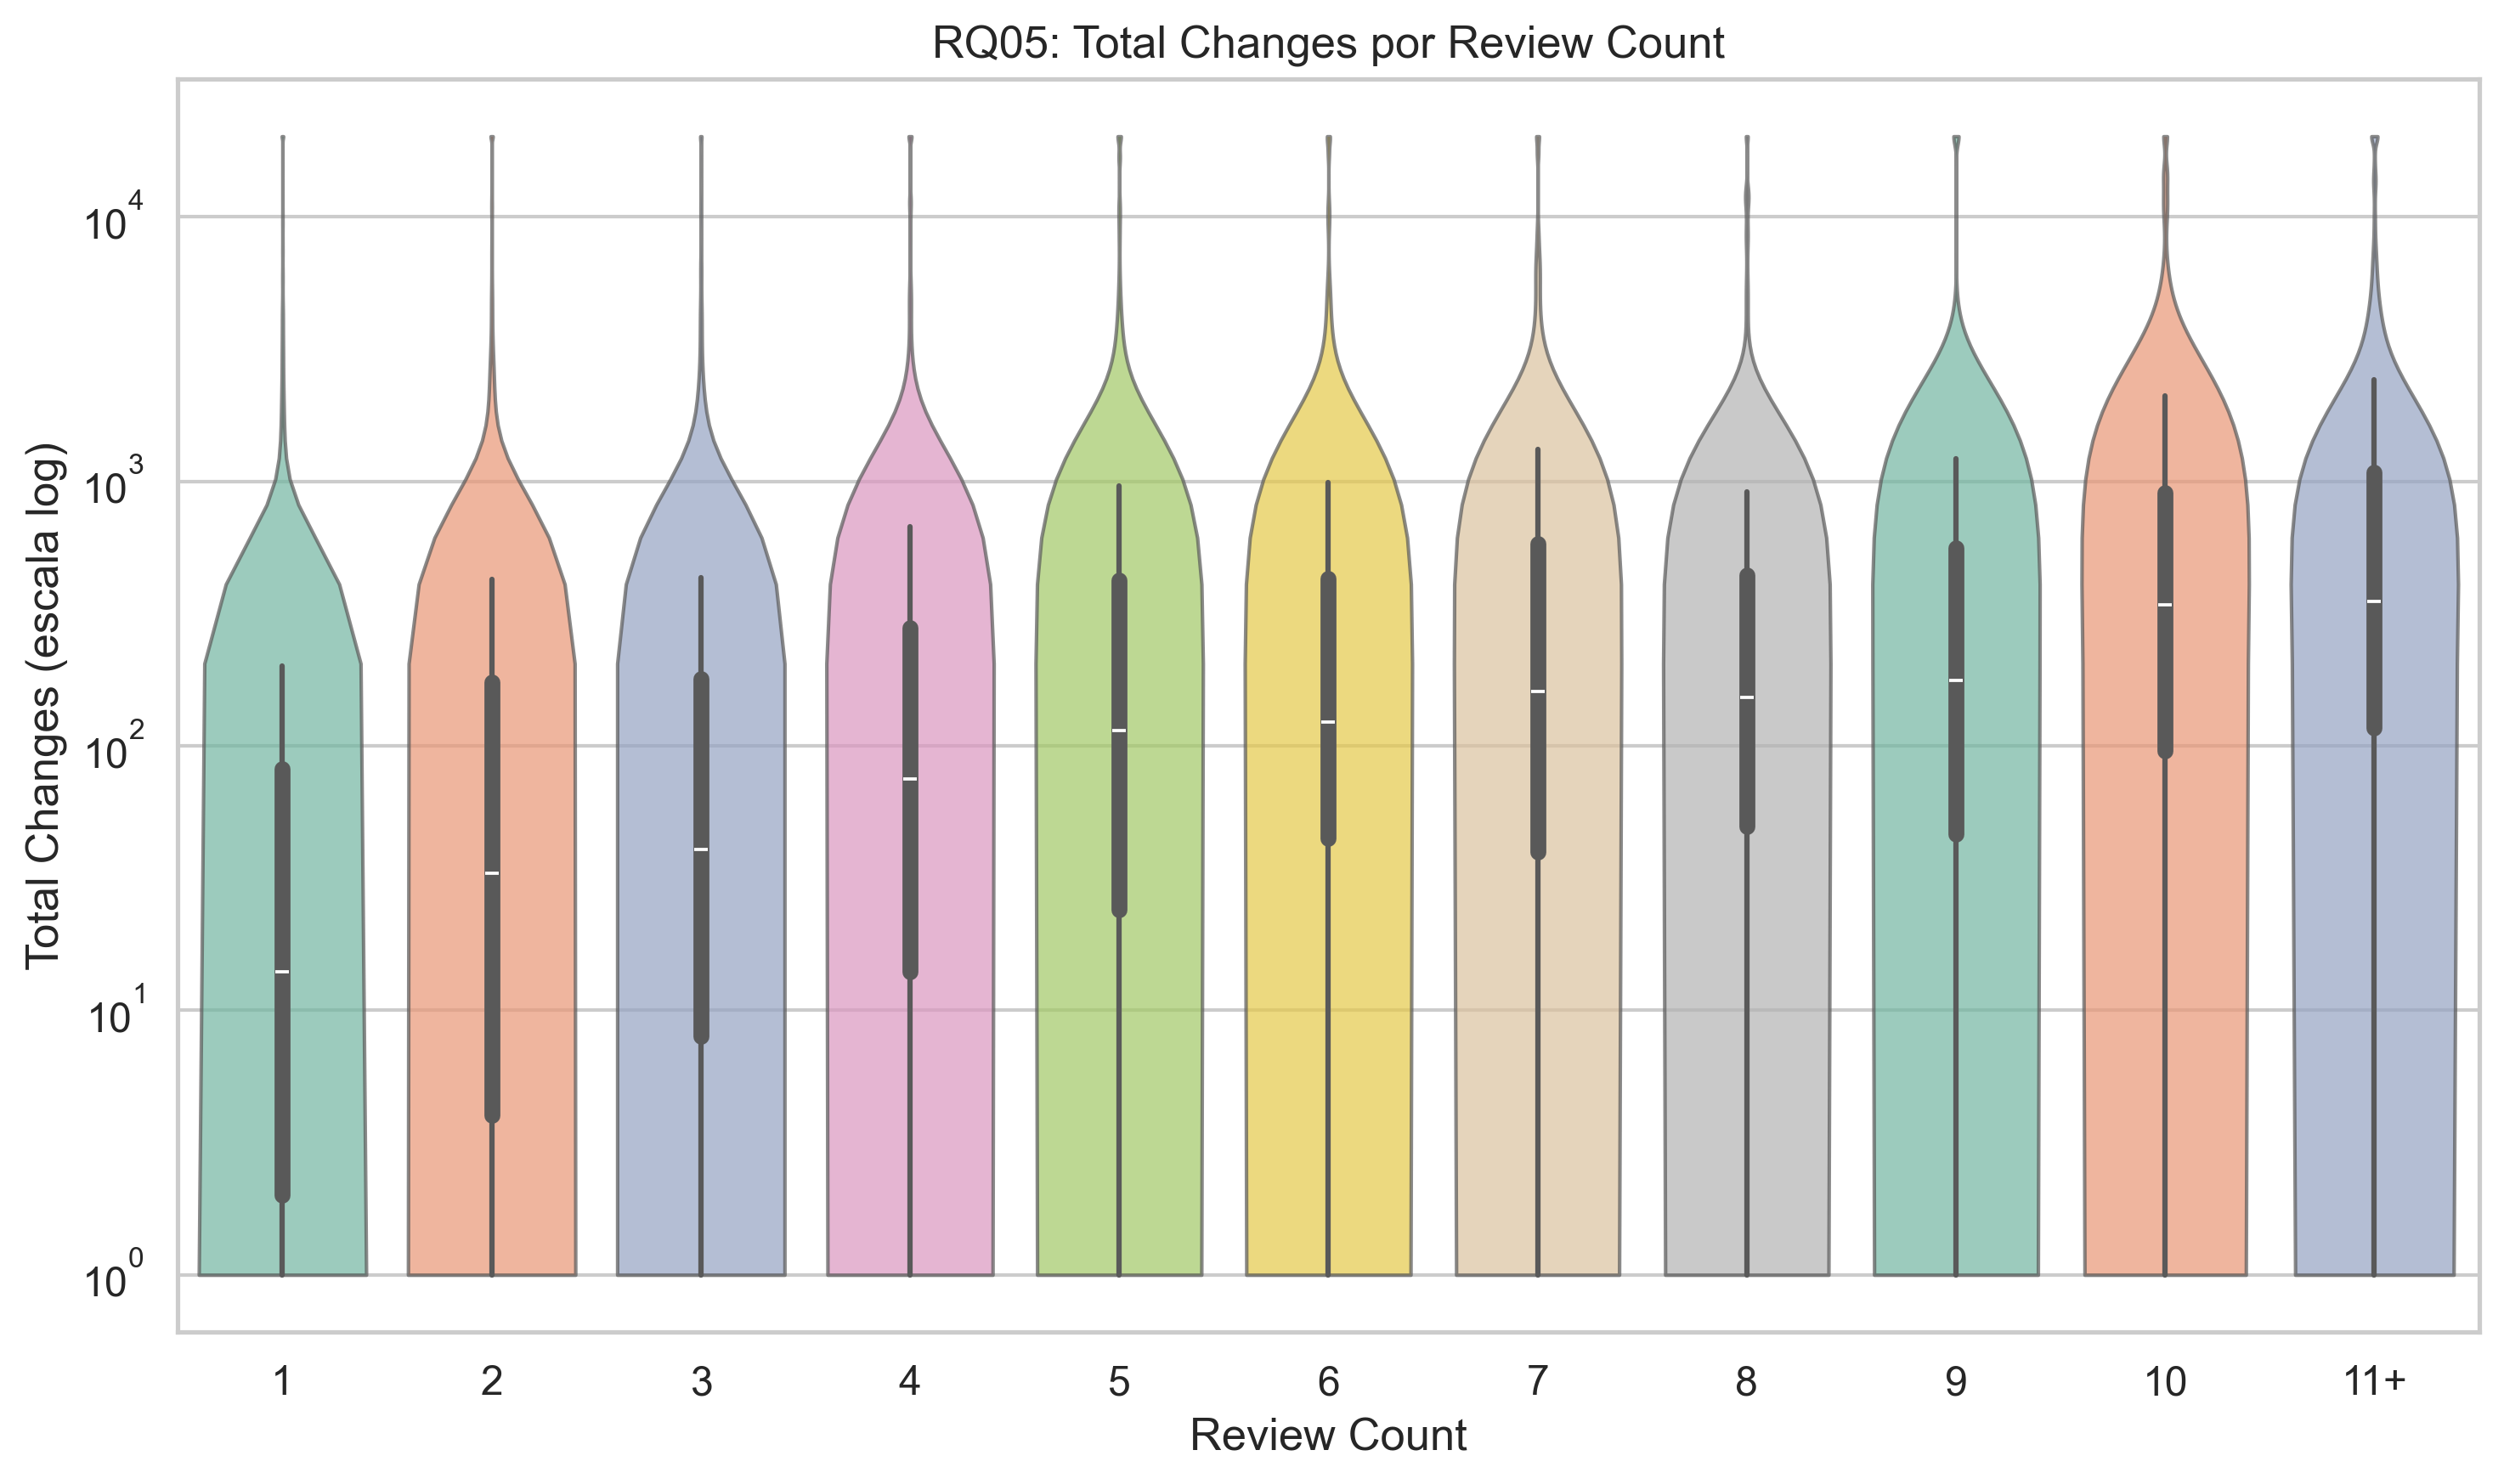
\includegraphics[width=0.85\textwidth]{figures/rq05.png}
    \caption{RQ05: Violin plot de tamanho do PR por número de revisões.}
    \label{fig:rq05}
\end{figure}

\subsubsection{RQ06 -- Tempo vs. Revisões}
Correlação desprezível ($\rho = 0,0917$, $p < 0,0001$).
Tempo de análise não aumenta sistematicamente com número de revisões.

\begin{figure}[H]
    \centering
    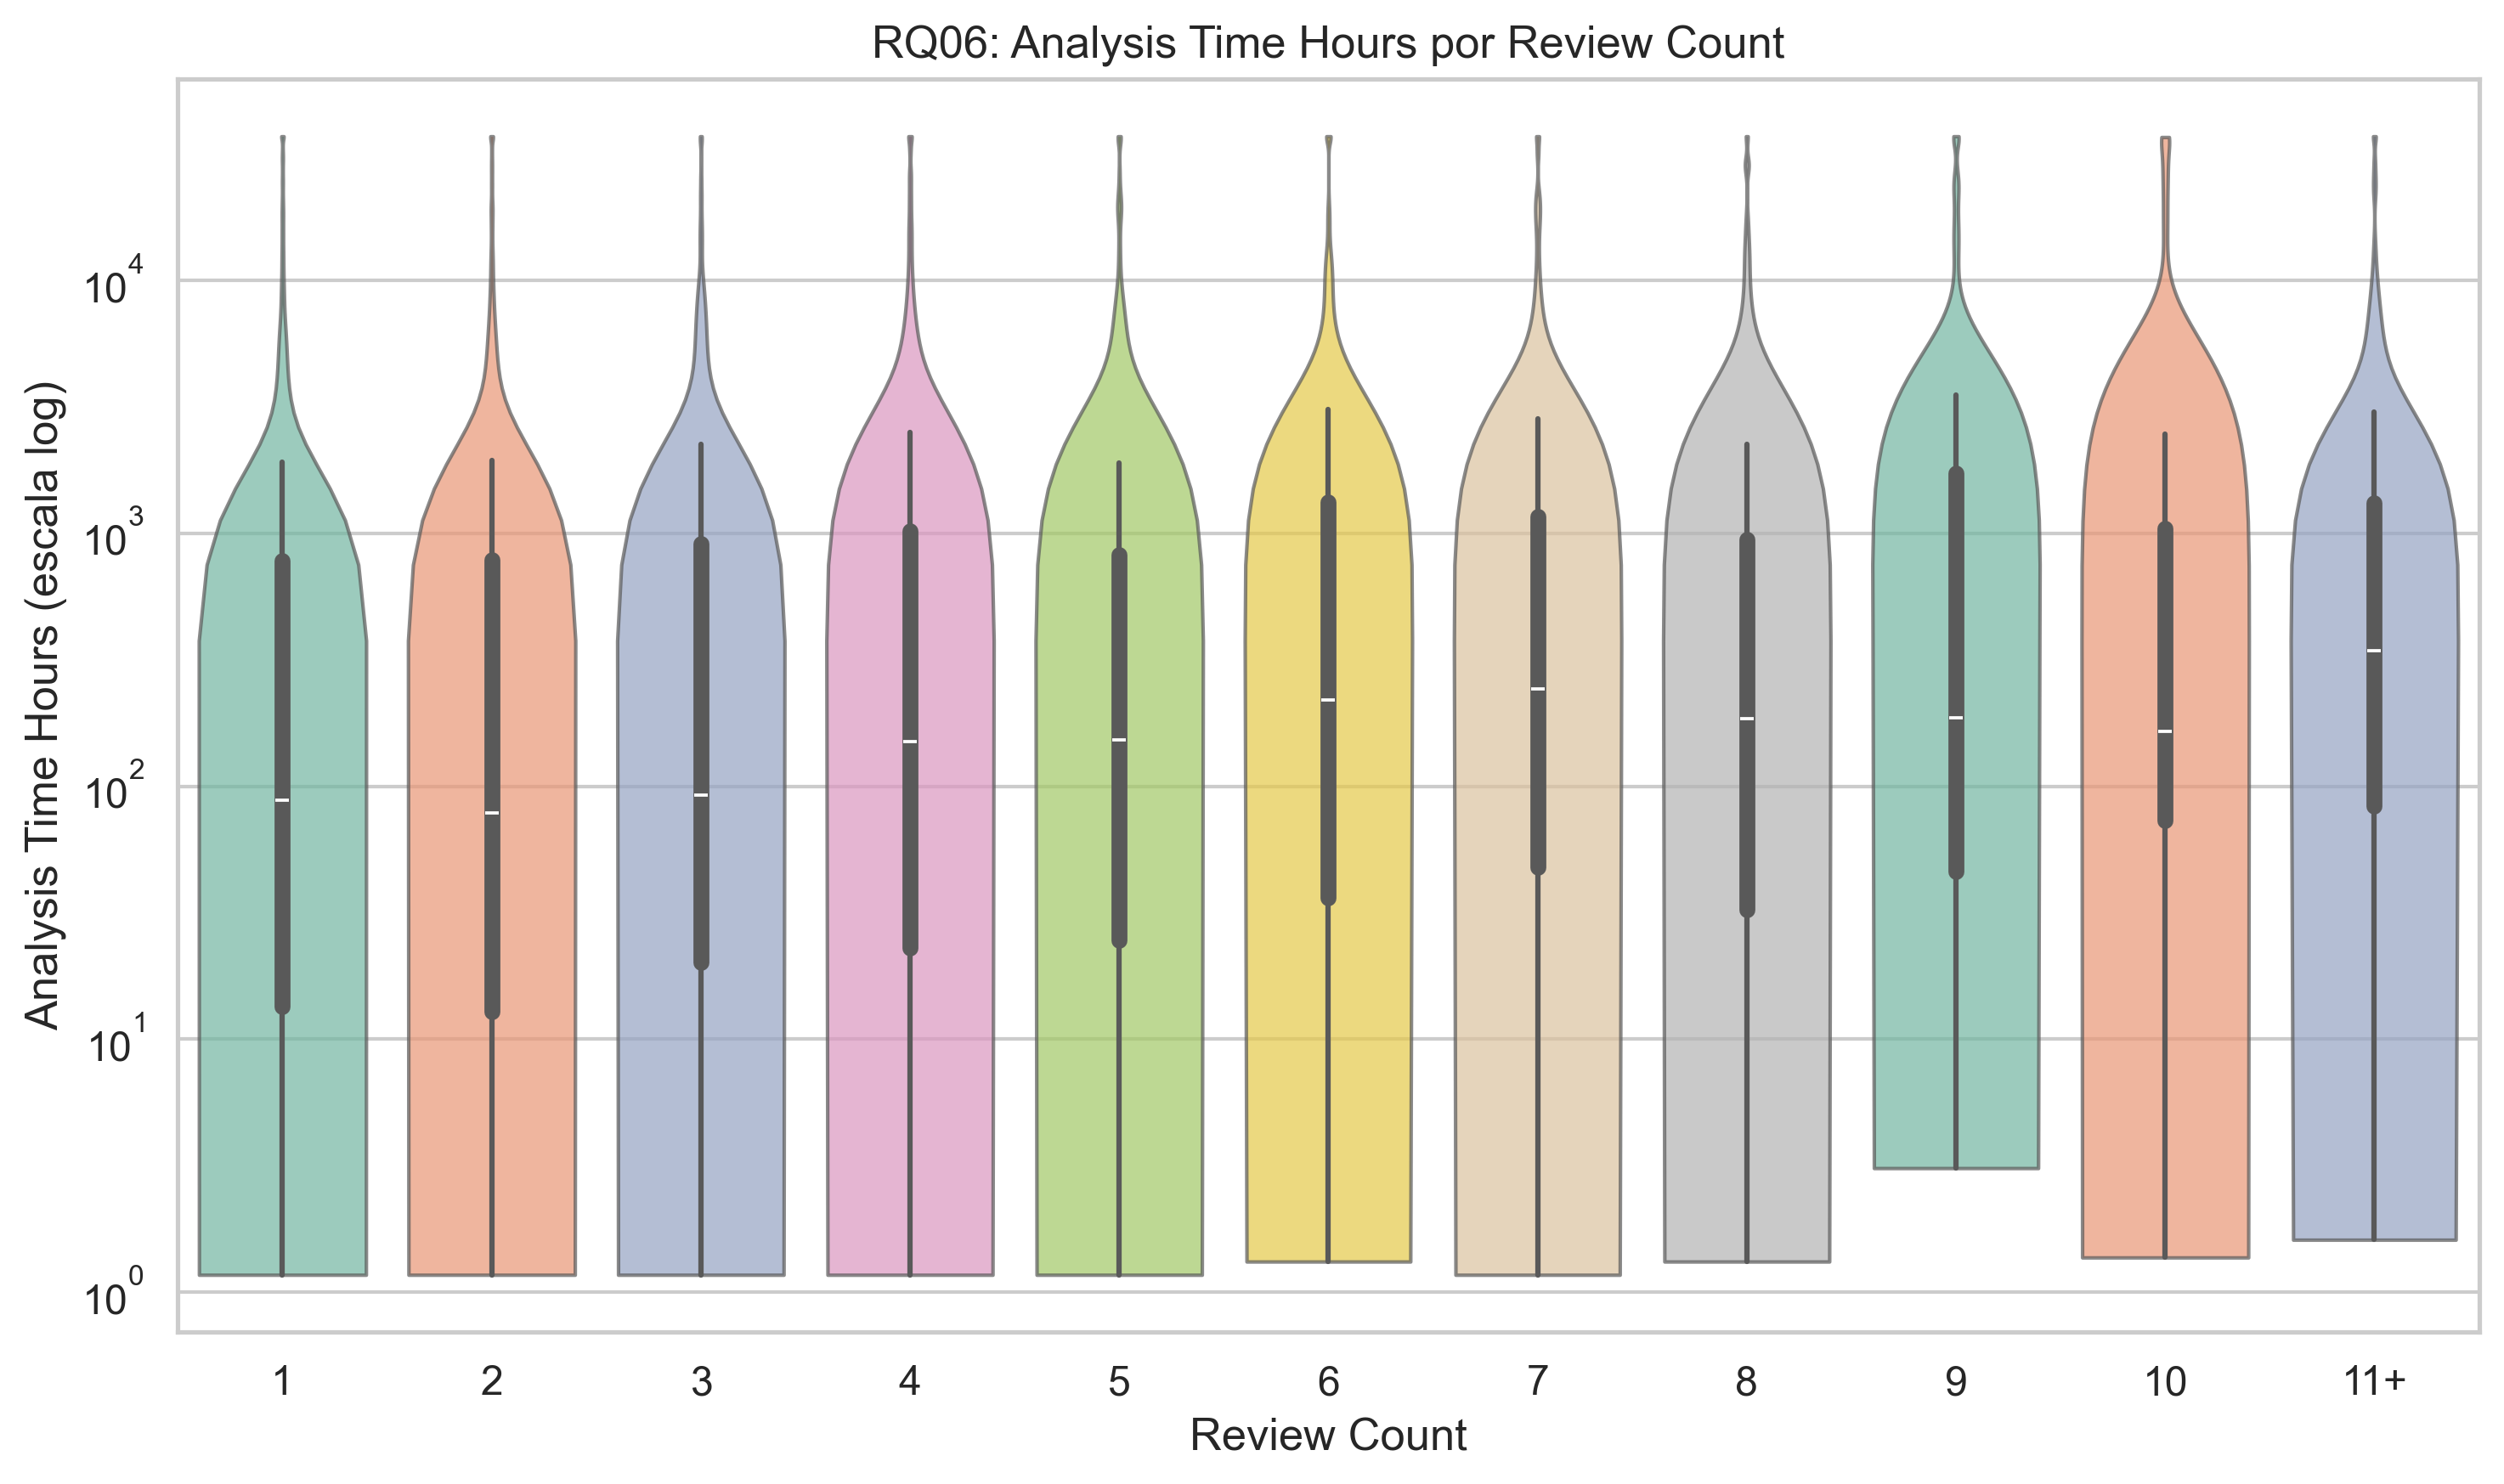
\includegraphics[width=0.85\textwidth]{figures/rq06.png}
    \caption{RQ06: Violin plot de tempo de análise por número de revisões.}
    \label{fig:rq06}
\end{figure}

\subsubsection{RQ07 -- Descrição vs. Revisões}
Correlação fraca ($\rho = 0,1861$, $p < 0,0001$).
Descrições maiores tendem a receber ligeiramente mais revisões.

\begin{figure}[H]
    \centering
    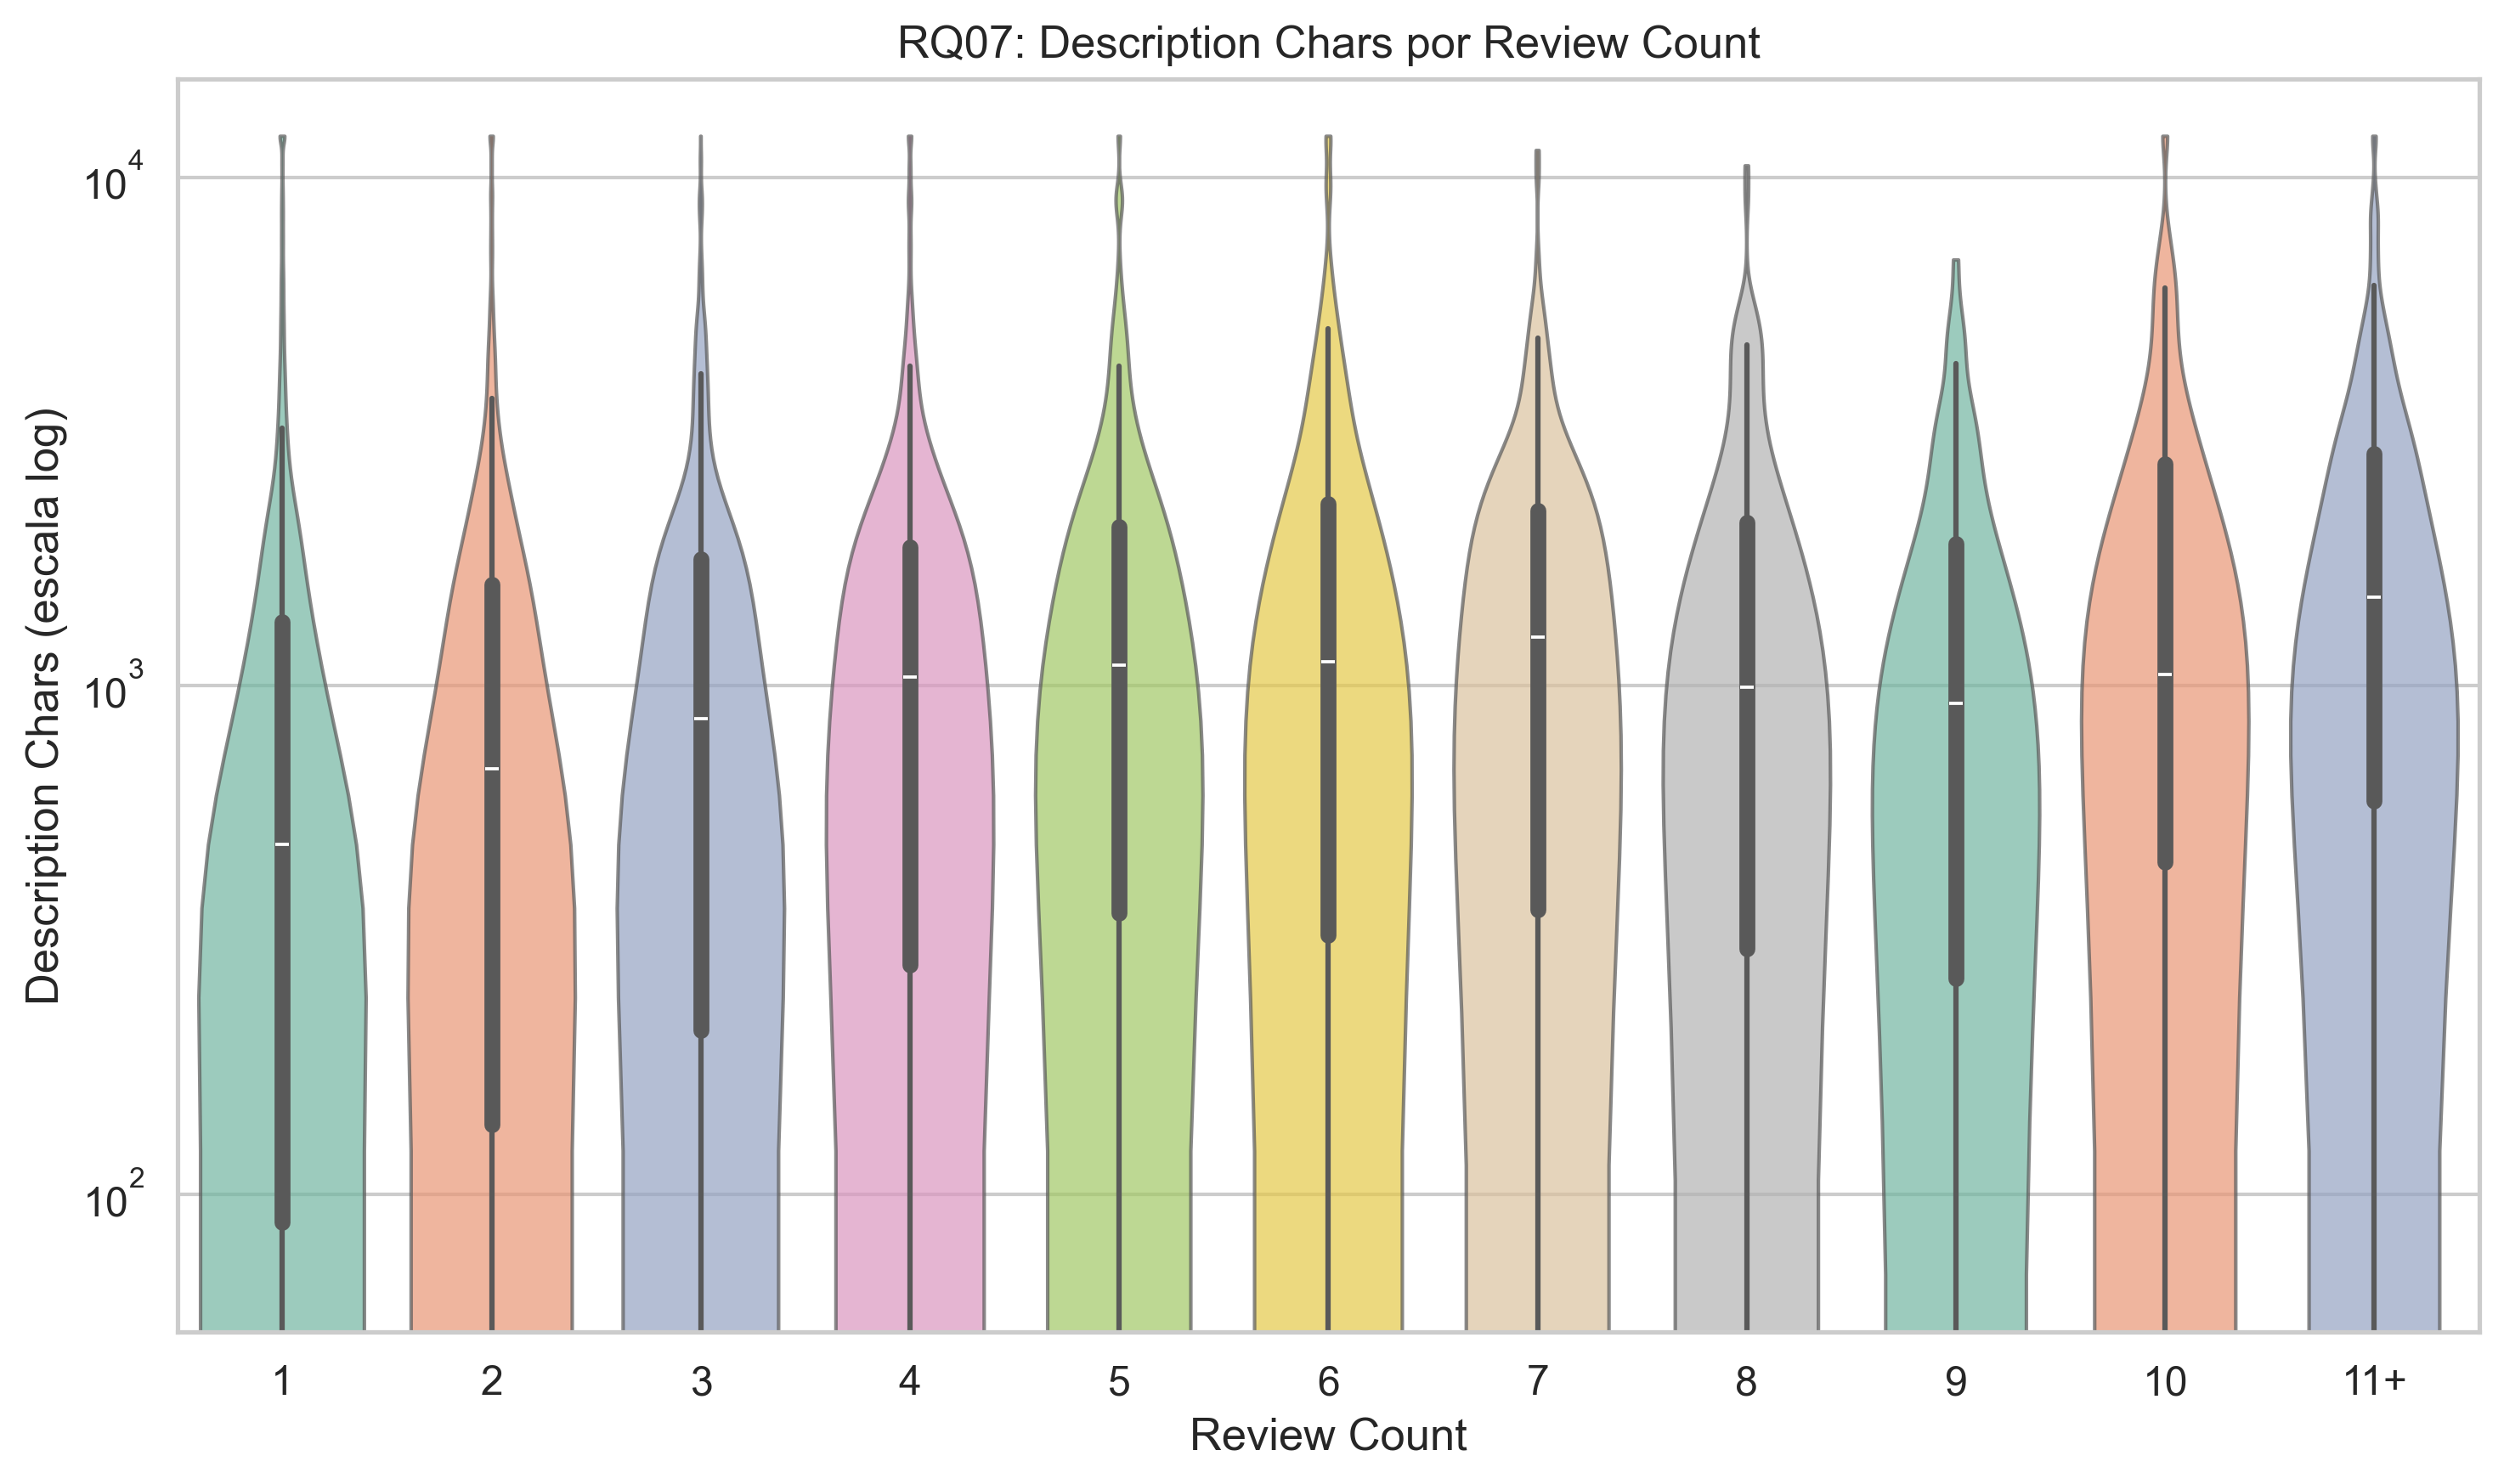
\includegraphics[width=0.85\textwidth]{figures/rq07.png}
    \caption{RQ07: Violin plot de tamanho da descrição por número de revisões.}
    \label{fig:rq07}
\end{figure}

\subsection{Matriz de Correlação}

A matriz de correlações entre todas as métricas revela a forte correlação
entre \texttt{lines\_added} e \texttt{total\_changes} ($\rho = 0,97$),
confirmando que são medidas redundantes.

\begin{figure}[H]
    \centering
    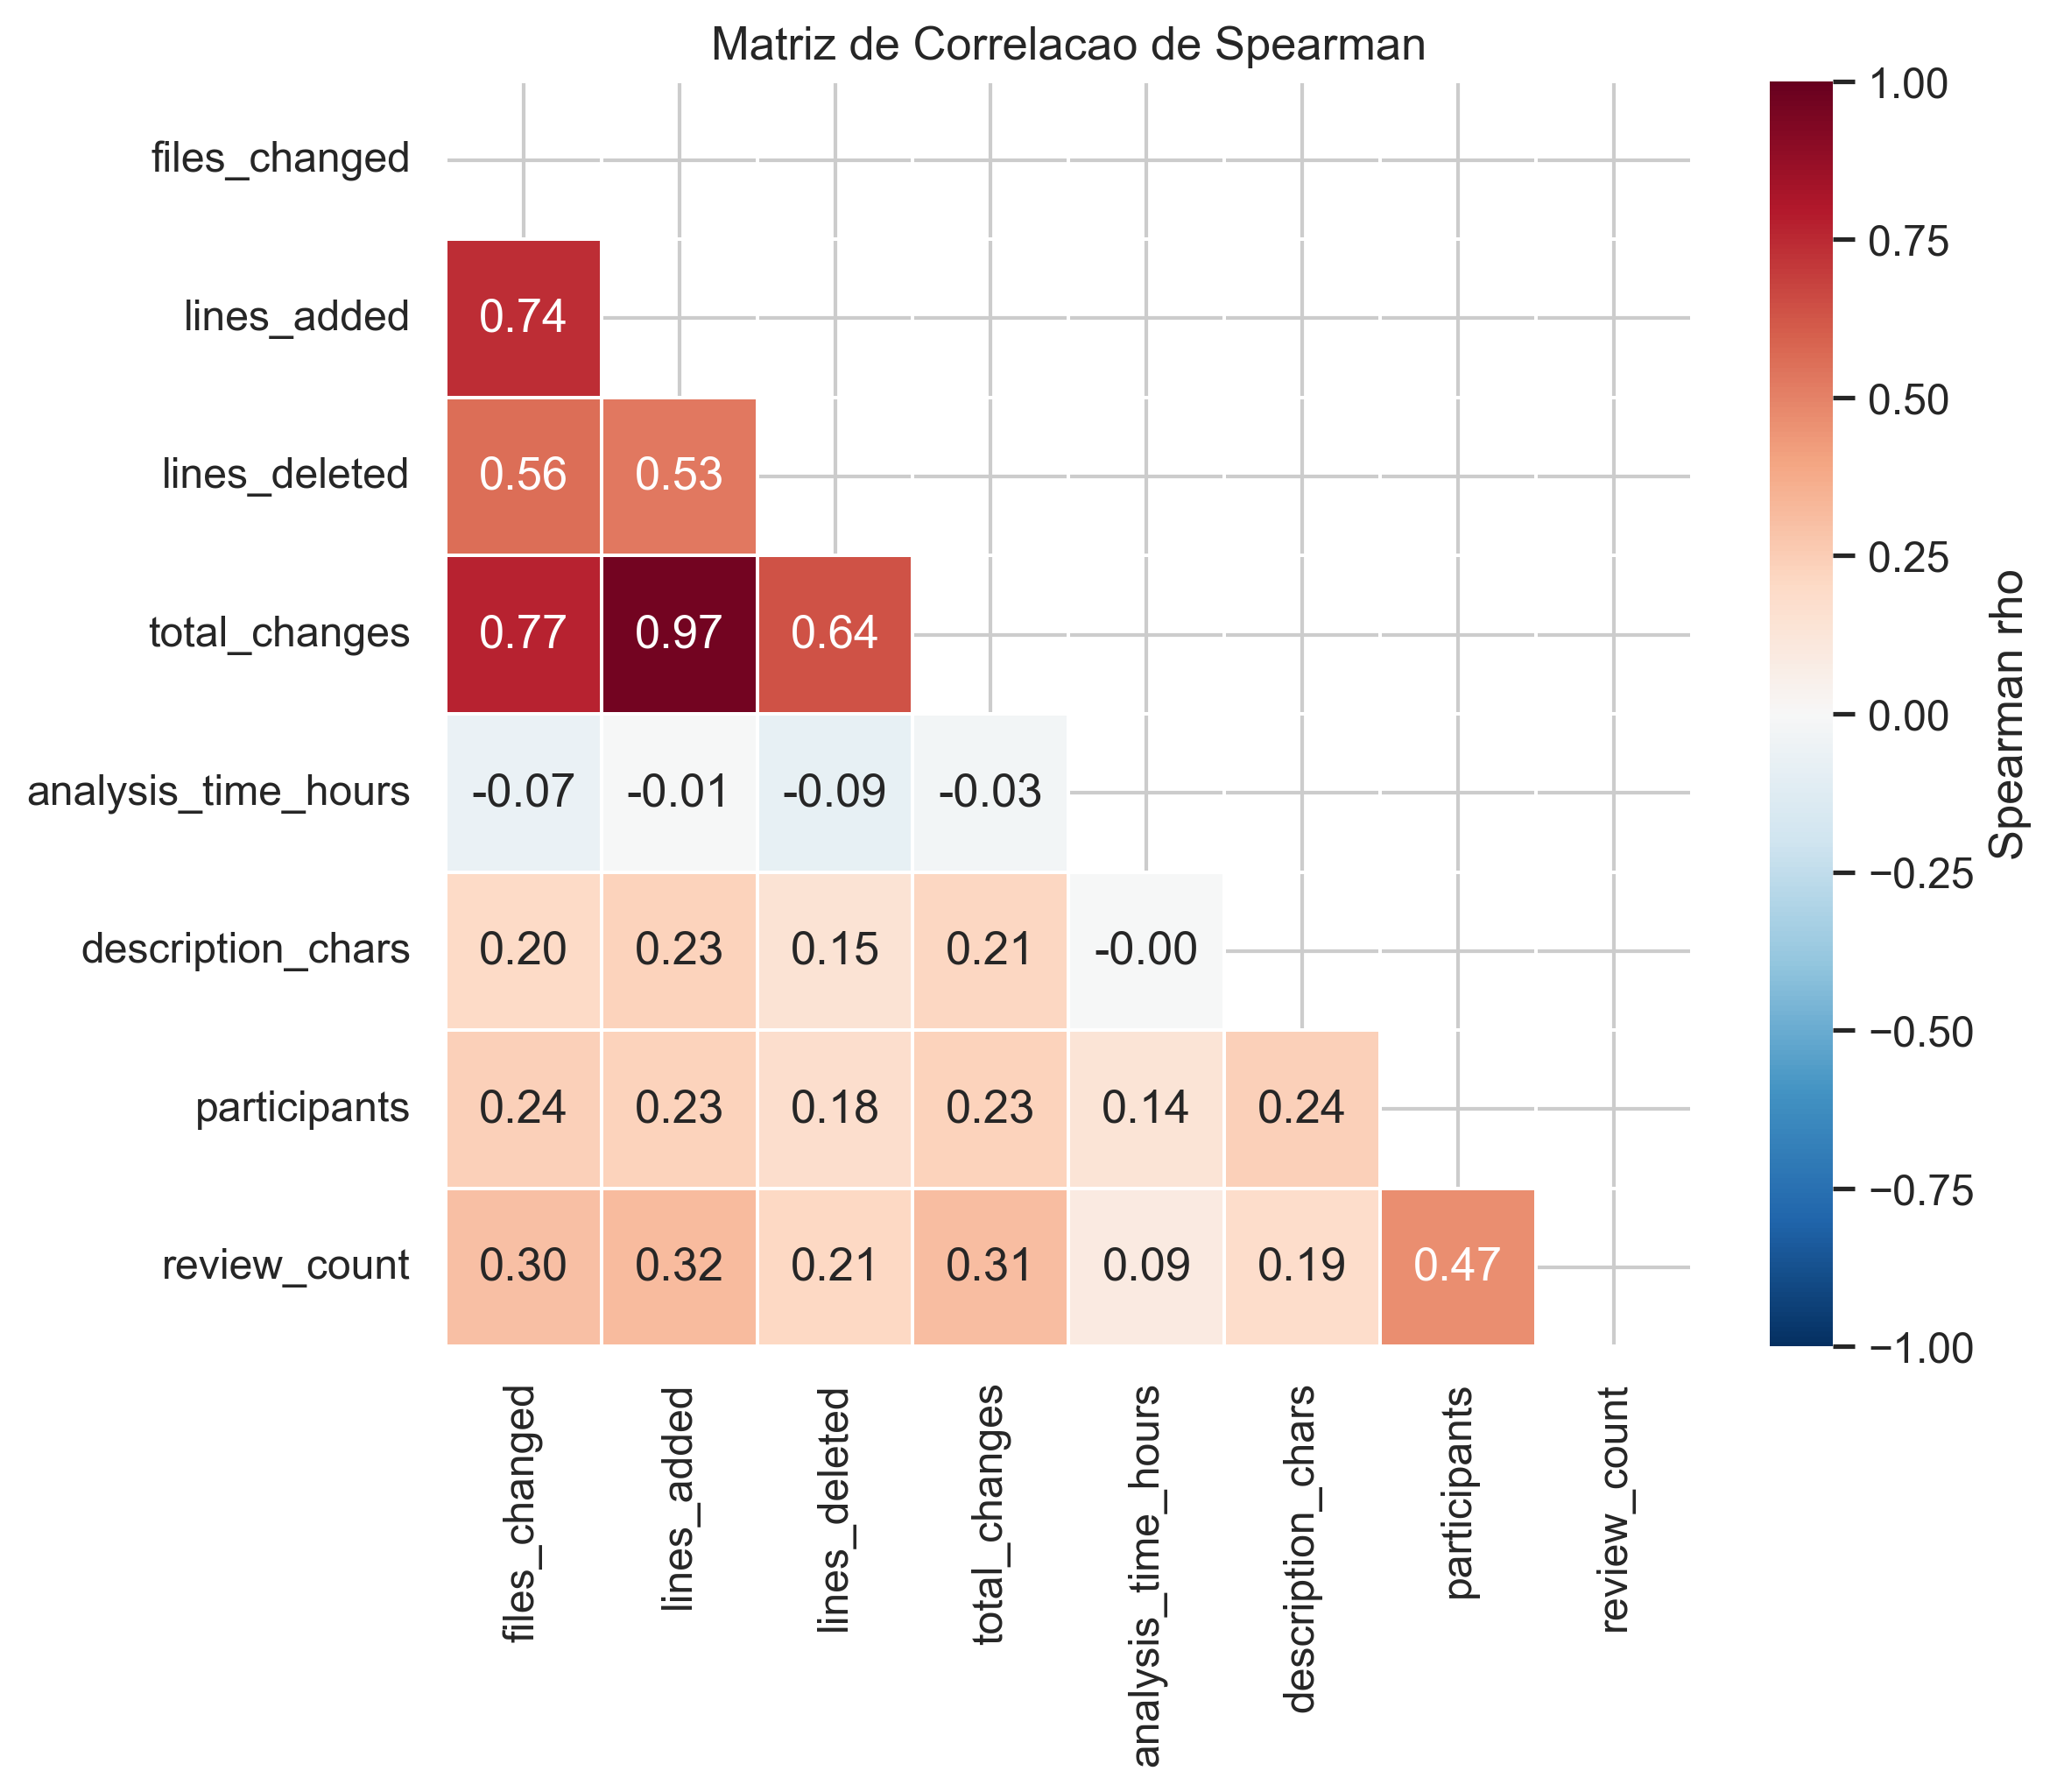
\includegraphics[width=\textwidth]{figures/correlation_matrix.png}
    \caption{Matriz de correlação de Spearman entre todas as métricas.}
    \label{fig:corr}
\end{figure}

\subsection{Distribuições Gerais}

As distribuições de todas as métricas por status de merge, apresentadas
em ECDF, mostram que a diferença mais marcante está no tempo de análise.

\begin{figure}[H]
    \centering
    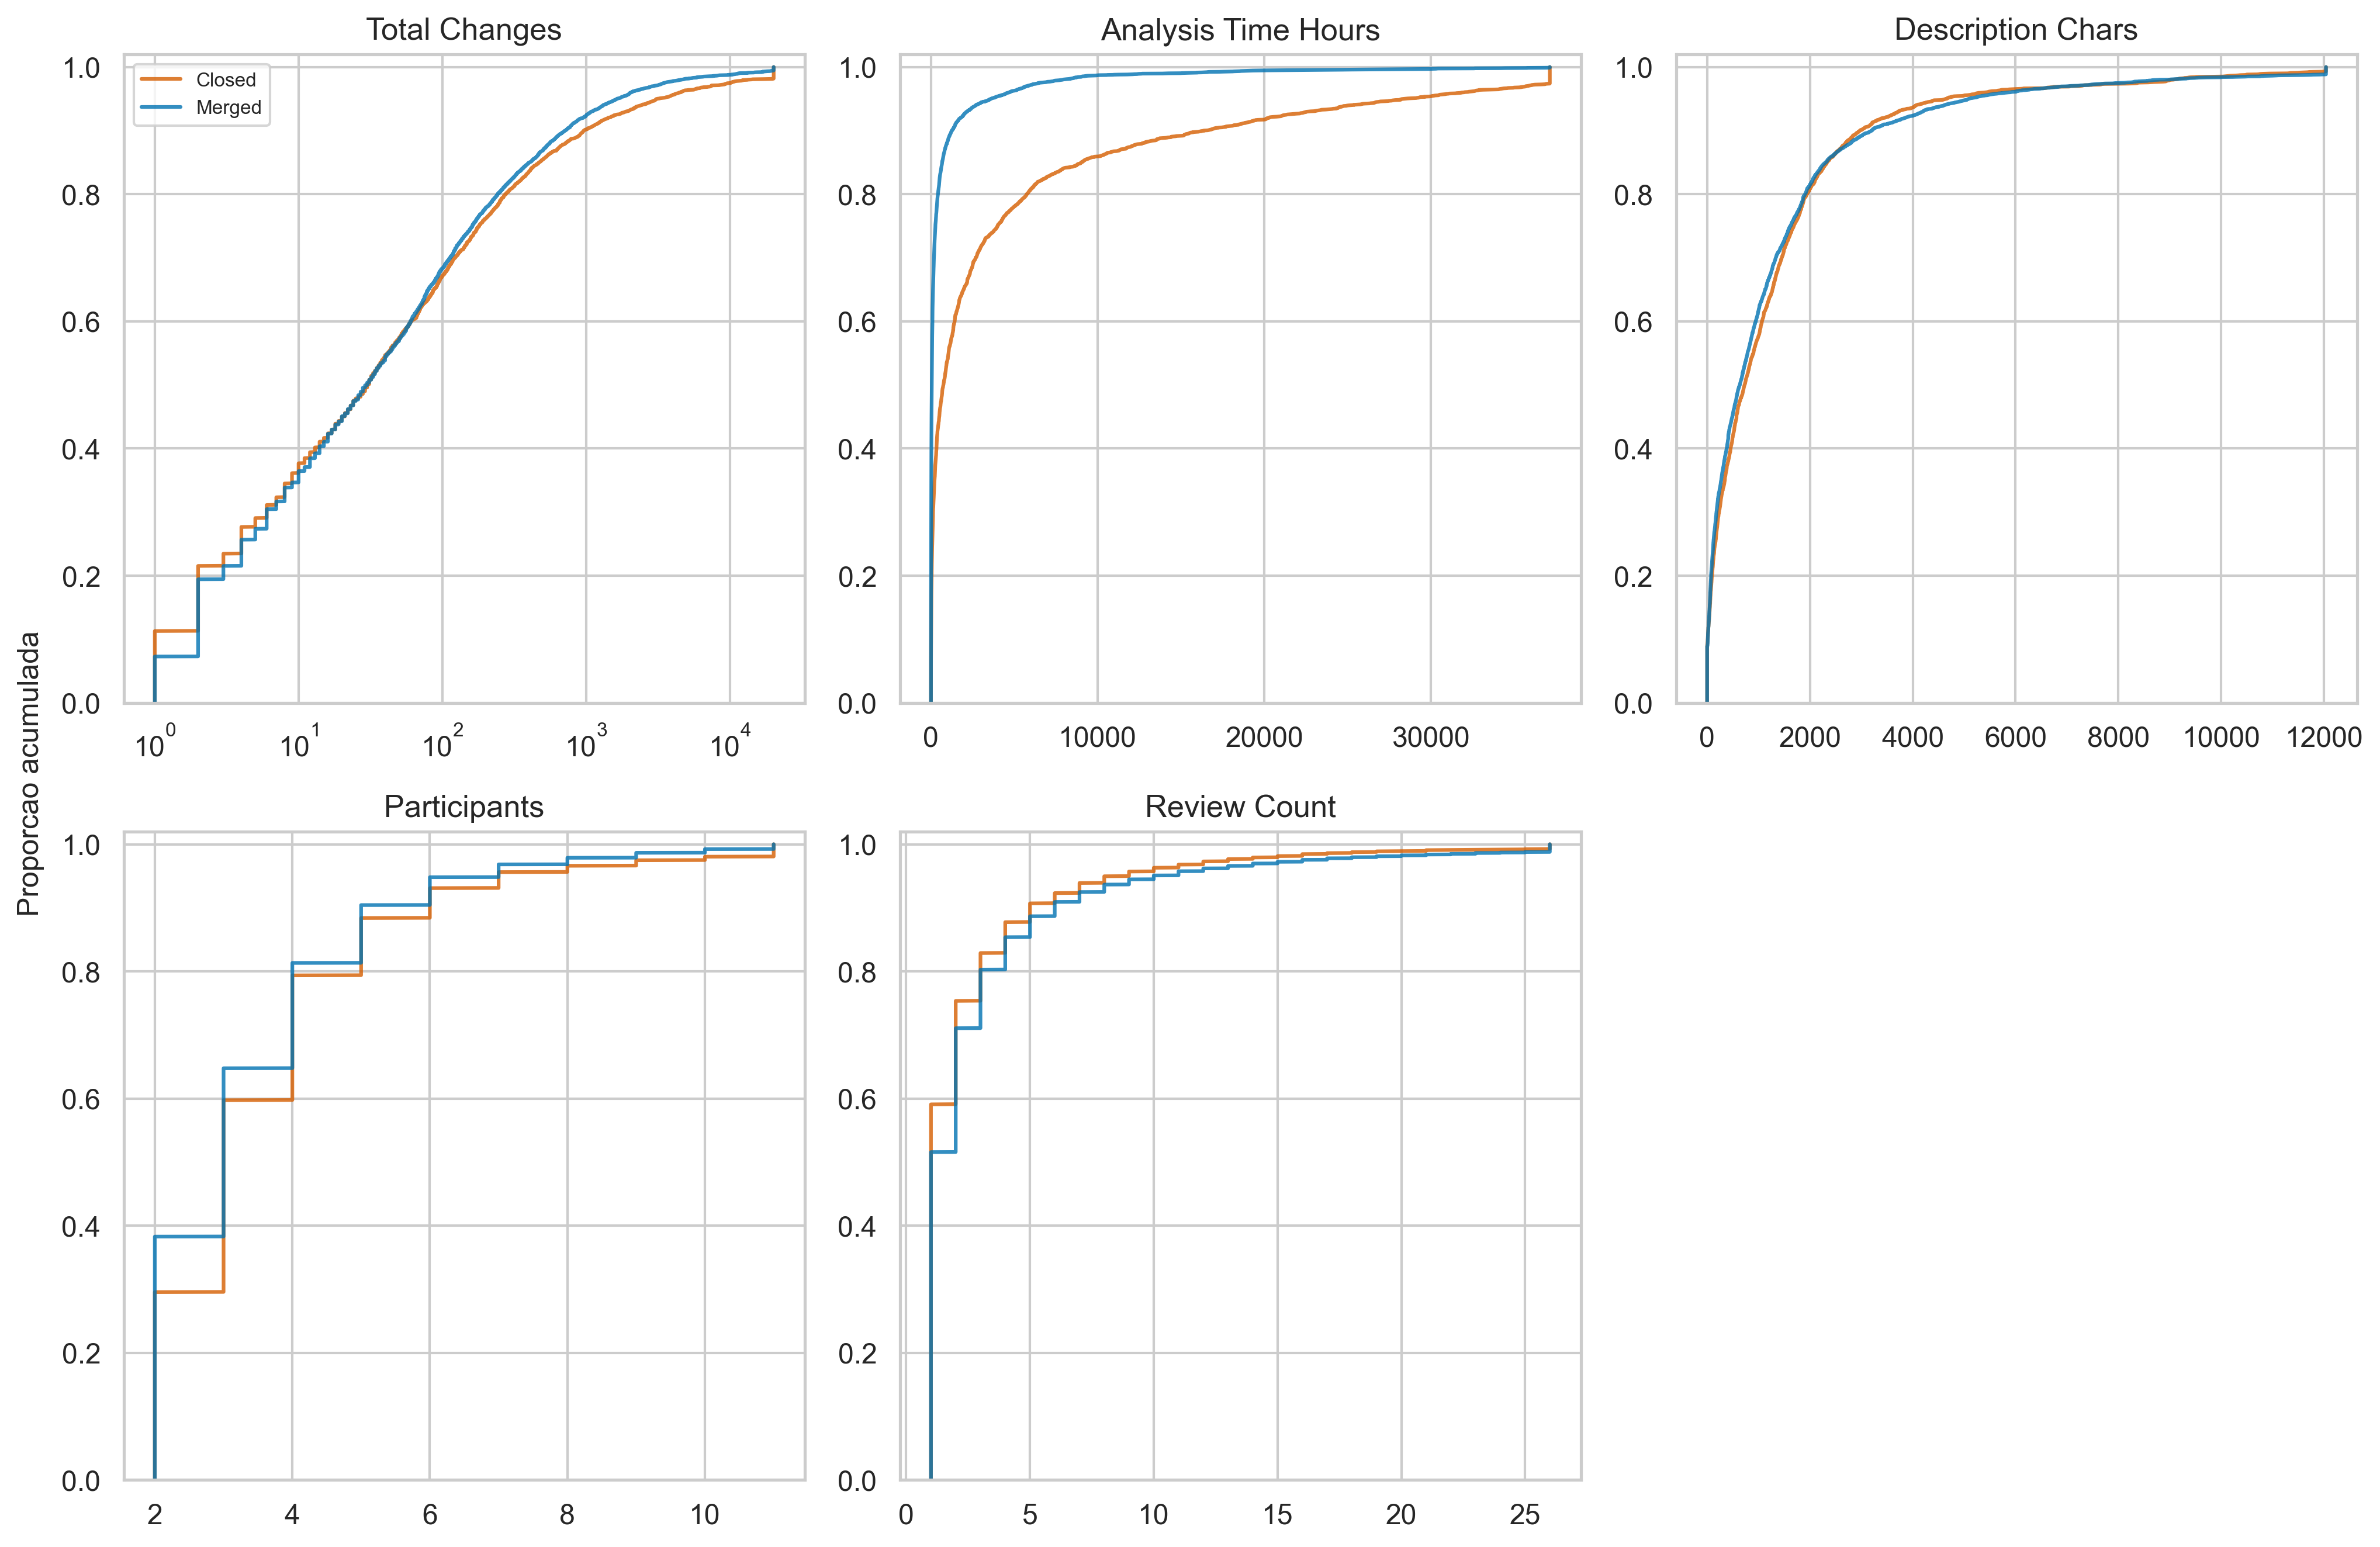
\includegraphics[width=\textwidth]{figures/distribution_ecdf.png}
    \caption{ECDF de todas as métricas por status de merge.}
    \label{fig:ecdf}
\end{figure}

\subsection{Revisões por Status}

PRs merged tendem a ter mediana de 1 revisão, enquanto closed têm mediana de 2.

\begin{figure}[H]
    \centering
    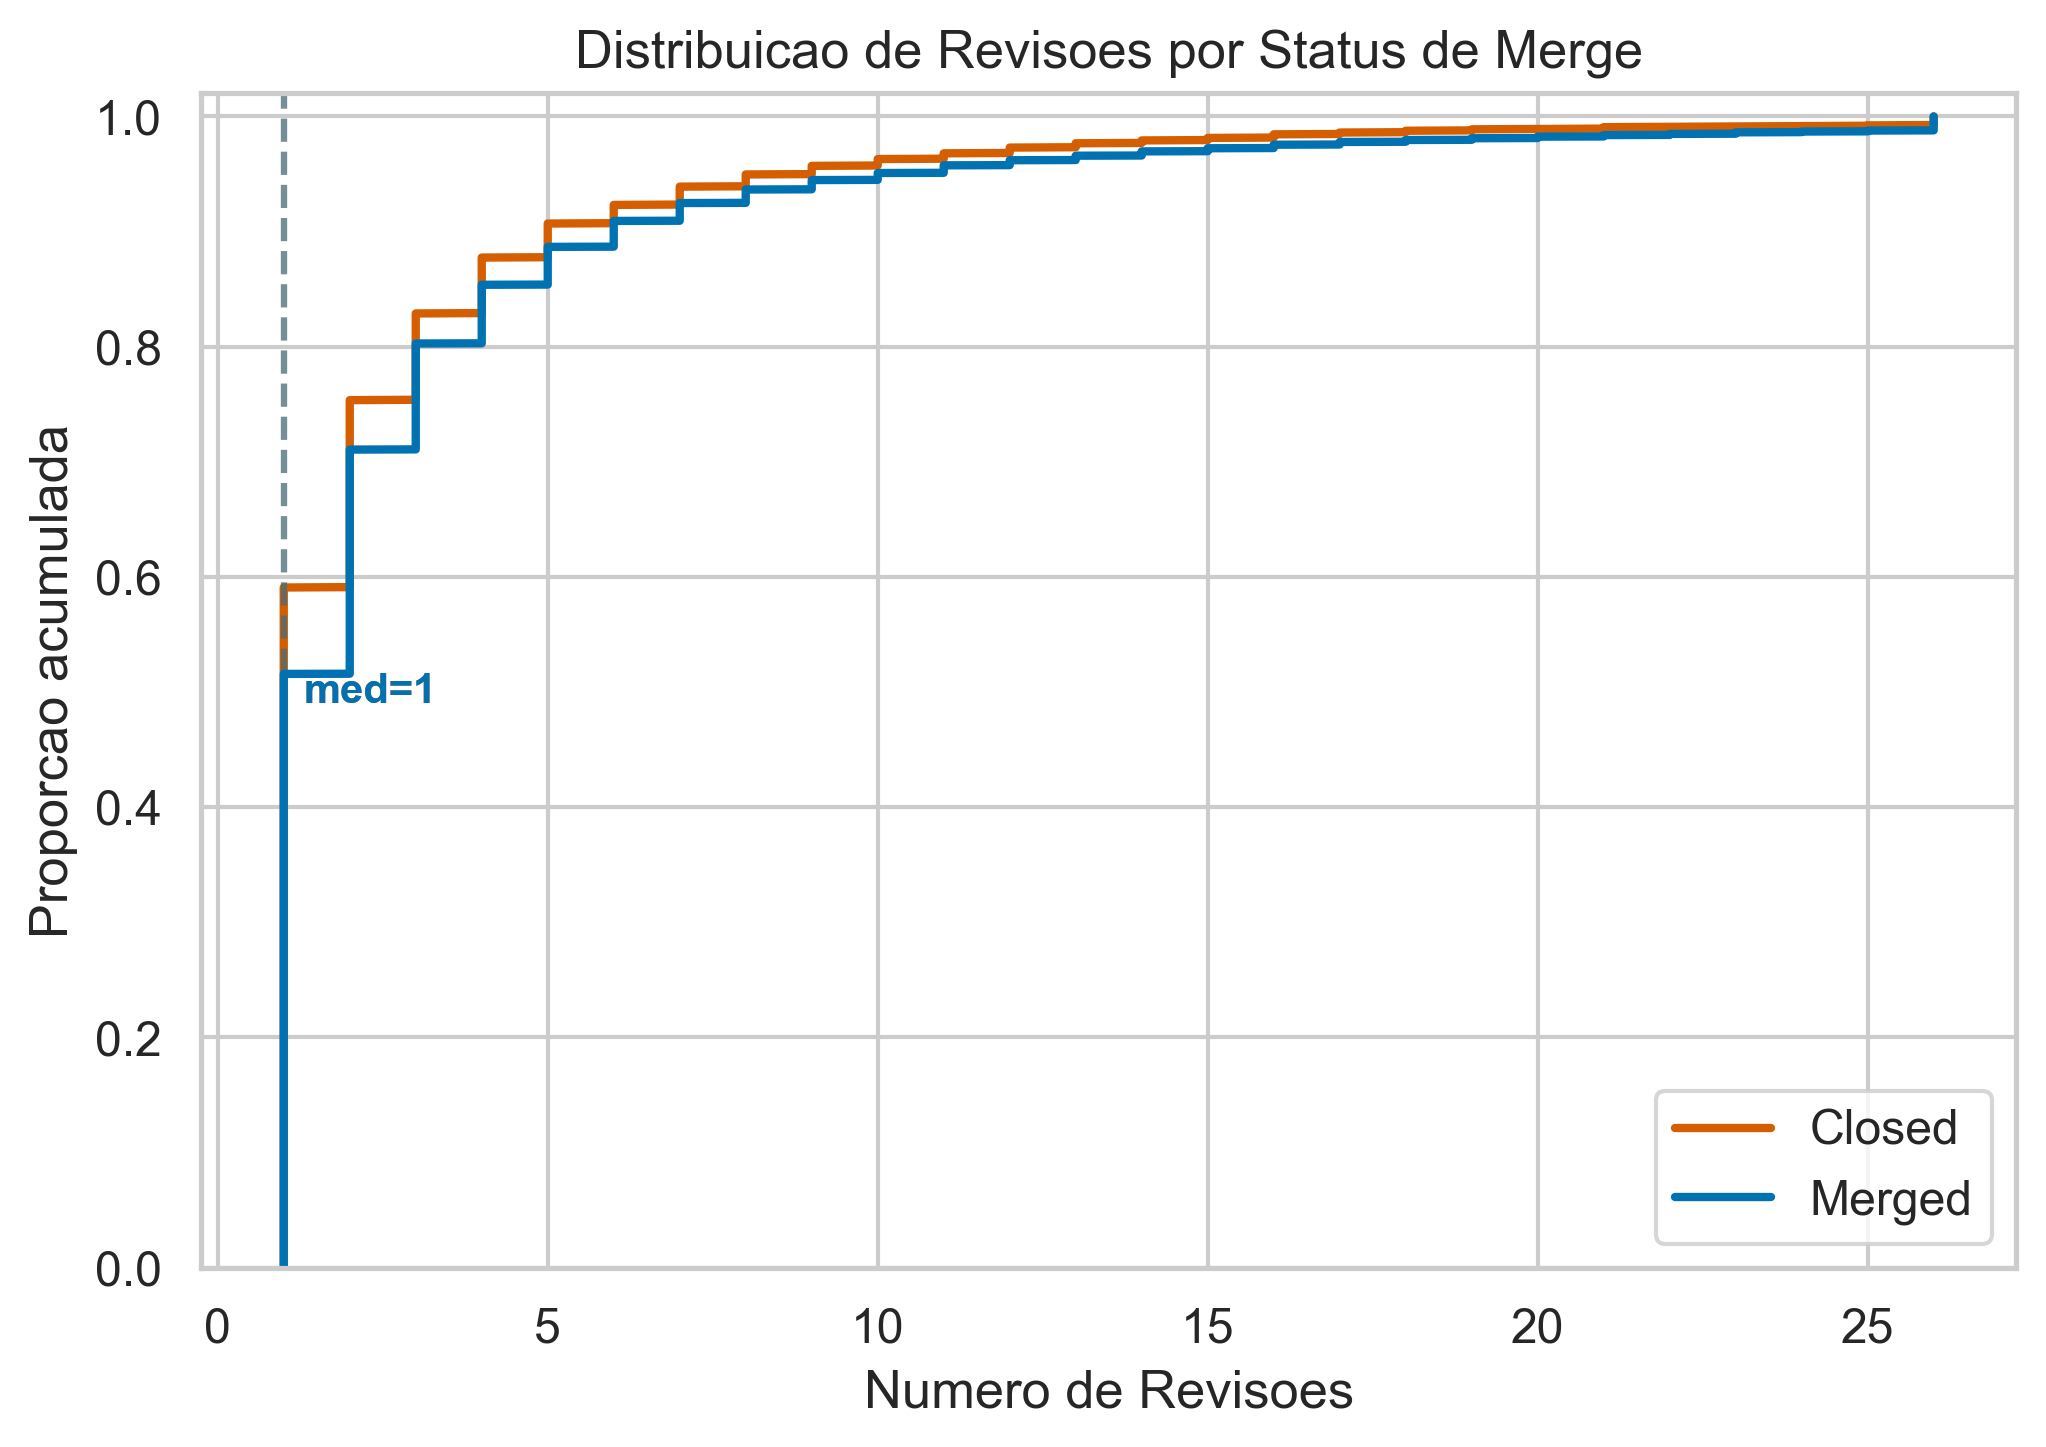
\includegraphics[width=0.85\textwidth]{figures/merged_vs_reviews.png}
    \caption{ECDF do número de revisões por status de merge.}
    \label{fig:reviews}
\end{figure}
